\author{João Gonçalves} %hallo adoro-te muito (⁠ ⁠˘⁠ ⁠³⁠˘⁠)⁠♥
\newcommand{\authorr}{Teresa Nogueira}
\newcommand{\studentID}{99995}
\newcommand{\studentIDD}{100029}
%\newcommand{\supervisorone}{Prof\textsuperscript{\underline{a}}. XXXXXX}
\newcommand{\supervisorone}{}
\newcommand{\supervisortwo}{}
\newcommand{\department}{Engenharia Eletrotécnica e de Computadores}
\newcommand{\exam}{Circuitos Electrónicos}

\title{%
Apontamentos sobre CEB\\
\large (Alguns tópicos \href{https://github.com/Kons-5}{\raisebox{0 em}{\large \faGithub}})}
\date{Maio 2023}

\documentclass[a4paper,12pt]{article}
\usepackage[left=25mm,top=21mm,right=25mm,bottom=21mm]{geometry}
\usepackage[flushmargin,hang,bottom,multiple]{footmisc}
\usepackage[usestackEOL]{stackengine}
\usepackage{babel}
\usepackage[T1]{fontenc}
\usepackage[utf8]{inputenc}
\usepackage{fontawesome5,textcomp}
\usepackage{xcolor}
\usepackage{fancyhdr}

\usepackage[export]{adjustbox}
\usepackage{graphicx,array,tabularx}
\usepackage{float,wrapfig}
\usepackage[font=footnotesize,labelfont=bf]{caption}
\usepackage[justification=centering]{subcaption}

\usepackage{amsmath,amsfonts,amssymb}
\usepackage{bm}
\usepackage{mathtools}
\usepackage{mathabx}
\usepackage{physics}
\usepackage{cancel}
\usepackage{empheq}

\usepackage{pgfplots}
\usepackage{msc}
\usepackage{booktabs}
\usepackage{tcolorbox}
\usepackage{etoolbox}

\usepackage{makecell}
\usepackage{listings}
\usepackage{enumitem}

\usepackage[linktoc=all]{hyperref}
\usepackage[capitalise]{cleveref}
\usepackage[nottoc,numbib]{tocbibind}
\usepackage[square,numbers,sort]{natbib}
\usepackage{breakurl}
\usepackage{placeins}
\usepackage{colortbl}
\usepackage{attrib}
\usepackage{multirow,multicol}

%\usepackage[printwatermark]{xwatermark}
\usepackage[framemethod=TikZ]{mdframed}
%\tcbuselibrary{skins,breakable}
%\usetikzlibrary{shadings,shadows}
\linespread{1}
%\setlength{\parindent}{0pt}

\hypersetup{
    colorlinks,
    linkcolor={black},
    citecolor={blue!50!black},
    urlcolor={blue!50!black}
}

\setlength{\abovedisplayskip}{3pt}
\setlength{\belowdisplayskip}{3pt}
\setlength{\fboxsep}{1.25\fboxsep}

\newcommand*\widefbox[1]{\fbox{\hspace{2em}#1\hspace{2em}}}

\let\zzzfootnotesize\footnotesize
\def\newfootnotesize{%
\zzzfootnotesize
\abovedisplayskip=0pt
\belowdisplayskip=\abovedisplayskip
\abovedisplayshortskip=\abovedisplayskip
\belowdisplayshortskip=\abovedisplayskip
}
\renewcommand\footnotesize{\protect\newfootnotesize}

\mdfsetup{%
    linewidth=2pt
}
%//==============================--@--==============================//%
%                         -> error messages <-                        %
\usepackage{pifont}

\newenvironment{warning}
  {\par\begin{mdframed}[linewidth=1.5pt,linecolor=red]%
    \begin{list}{}{\leftmargin=0.9cm
                   \labelwidth=\leftmargin}\item[\raisebox{-0.4 em}{\Large\ding{43}}]}
  {\end{list}\end{mdframed}\par}

%//==============================--@--==============================//%
%                   -> reduzir espaço entre itens <-                  %
\usepackage{enumitem}
%\setlist[itemize]{nosep}
%\setlist[enumerate]{nosep}
\setlist[itemize]{itemsep=0.0125em}
\setlist[enumerate]{itemsep=0.0125em}
%//==============================METH-==============================//%
\newcounter{theo}[section]\setcounter{theo}{0}
\renewcommand{\thetheo}{\arabic{theo}}

%\definecolor{tempcolor}{RGB}{113, 110, 97}
\definecolor{tempcolor}{RGB}{0, 0, 0}
\newenvironment{theo}[2][]{%
    \refstepcounter{theo}
    \ifstrempty{#1}%
    % if condition (without title)
    {\mdfsetup{%
        frametitle={%
            \tikz[baseline=(current bounding box.east),outer sep=0pt]
            \node[anchor=east,rectangle,fill=blue!20]
            {\strut Teorema~\thetheo};}
        }%
    % else condition (with title)
    }{\mdfsetup{%
        frametitle={%
            \tikz[baseline=(current bounding box.east),outer sep=0pt]
            \node[anchor=east,rectangle,fill=white]
            {\strut #1};}%
        }%
    }%
    % Both conditions
    \mdfsetup{%
        innertopmargin=0pt,linecolor=tempcolor,%
        linewidth=2pt,topline=true,%
        frametitleaboveskip=1.25\dimexpr-\ht\strutbox\relax%
    }
 
\begin{mdframed}[]\relax\vspace{-0.5em}}{%
\end{mdframed}}

\def\delequal{\mathrel{\ensurestackMath{\stackon[1pt]{=}{\scriptstyle\Delta}}}}

\let\originalleft\left
\let\originalright\right
\renewcommand{\left}{\mathopen{}\mathclose\bgroup\originalleft}
\renewcommand{\right}{\aftergroup\egroup\originalright}
%------------------------------------ MAGIC--------------------------------------
\def\UrlBreaks{\do\/\do-}
\expandafter\def\expandafter\UrlBreaks\expandafter{\UrlBreaks\do\a%
\do\b\do\c\do\d\do\e\do\f\do\g\do\h\do\i\do\j\do\k\do\l\do\m\do\n%
\do\o\do\p\do\q\do\r\do\s\do\t\do\u\do\v\do\w\do\x\do\y\do\z\do\&}

\newcolumntype{C}[1]{>{\centering\let\newline\\\arraybackslash\hspace{0pt}}m{#1}}
\newcolumntype{L}[1]{>{\raggedright\let\newline\\\arraybackslash\hspace{0pt}}m{#1}}
%----------------------------------TITLE PAGE -----------------------------------
\makeatletter
\def\maketitle{
  \begin{center}\leavevmode
        \normalfont
        
\includegraphics[width=0.5\columnwidth]{img/title-page/IST.pdf}
        \vskip 0.05cm   
        \textsc{\large \department}\\
        \vskip 0.5cm
        \rule{0.95\linewidth}{0.2 mm} %\\
        {\large \exam}\\[0.5 cm]
        {\huge \bfseries \@title \par} 
        \vspace{1em}
        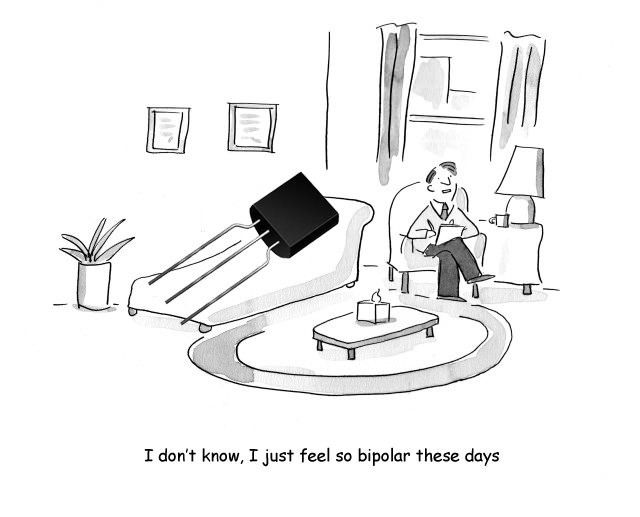
\includegraphics[scale=0.4]{img/title-page/000.png}
        %\vspace{0.5cm}
        \rule{0.95\linewidth}{0.2 mm} \\[0.75 cm]
        %\fontsize{9pt}{11pt}\selectfont
        \begin{minipage}[t]{1\textwidth}
	   \begin{flushleft} \large
                \emph{Autores:}\\
			\normalsize \textbf{\@author} : \studentID\\
                \fontsize{9pt}{11pt}\selectfont $\hookrightarrow$ jrazevedogoncalves@tecnico.ulisboa.pt \\
                \normalsize \textbf{\authorr} : \studentIDD\\
                \scriptsize $\hookrightarrow$ maria.teresa.ramos.nogueira@tecnico.ulisboa.pt
		\end{flushleft}
	\end{minipage}

    \vfill
	{\Large \@date\par}
   \end{center}
   %\vfill
   %\null
   \cleardoublepage
  }
\makeatother
%-------------------------------- ENDTITLE PAGE ----------------------------------
%---> Header <---
%\fancyhf{}
\renewcommand{\headrulewidth}{1pt}% Header rule width
\renewcommand{\footrulewidth}{0pt}% No footer rule
\setlength\headheight{26pt} 
\fancyhead[L]{\raisebox{0.1\height}[0pt][0pt]{\textit{Circuitos Electrónicos}}}
\fancyhead[R]{\raisebox{0.1\height}[0pt][0pt]{2022/2023}}
%%%%%%%%%%%%%%%%%

\pgfplotsset{compat=1.18}
\setcounter{tocdepth}{3}
%\setcounter{secnumdepth}{4}
\setcounter{secnumdepth}{-2}

\renewcommand{\figurename}{Fig.}
\renewcommand{\tablename}{Tab.}
\renewcommand{\contentsname}{Índice}
\settocbibname{\raisebox{0em}{Referências}}
\setlength{\bibsep}{0.15em}%reduzir espaço entre refs.

%\renewcommand{\bibpreamble}{\vspace{-8em}}
\usepackage[titles]{tocloft}
\setlength{\cftbeforesecskip}{0.35em}

%\usepackage{pdfpages}
% \newwatermark[page=15,fontfamily=bch,color=red!50,angle=45,scale=3.5,xpos=-10,ypos=10]{TO BE ADDED}


\begin{document}
    \sloppy
    %% title page
    \pagenumbering{gobble}
    \maketitle
    %% toc
    \tableofcontents
    \setcounter{tocdepth}{4}
    %% body
    \newpage
    \pagestyle{fancy}
    \pagenumbering{arabic}

    % \clearpage
    % \section{Introdução}\label{sec:intro}%
    %     %//==============================--@--==============================//%

%//==============================--@--==============================//%

    \clearpage
    \section{1. Semicondutores}\label{sec:semiconductors}%
        %//==============================--@--==============================//%

Os semicondutores são materiais que possuem propriedades elétricas intermediárias entre os isolantes e os condutores, e dispõem de uma propriedade única: a sua condutividade eléctrica aumenta com a temperatura, ao contrário dos metais, cuja condutividade diminui com a temperatura. 

O silício (Si) e o germânio (Ge) são dois exemplos bem conhecidos de semicondutores (ambos do grupo 14 da tabela periódica).

%//==============================--@--==============================//%
\subsection[1.1 Semicondutores intrínsecos e dopados]{\hspace*{0.075 em}\raisebox{0.2 em}{$\pmb{\drsh}$} Semicondutores intrínsecos e dopados}
\label{subsec:semiconductors-intrinsic-and-doped}

\begin{itemize}
    \item \textbf{Semicondutores intrínsecos:} Semicondutores puros, como o silício cristalino, que não possuem impurezas. A condutividade elétrica é determinada apenas pela concentração de portadores de carga intrínsecos, ou seja, eletrões e lacunas geradas pela quebra de ligações covalentes.
    
    \item \textbf{Semicondutores dopados:} Semicondutores obtidos a partir da adição intencional de impurezas (dopantes) ao material semicondutor. O processo de dopagem permite controlar as propriedades elétricas do material e aumentar a sua condutividade. Existem dois tipos principais de dopagem de semicondutores:
    \begin{itemize}[label=$\blacktriangle$]
        \item \textbf{Dopagem de tipo n:} Dopagem com impurezas que possuem mais eletrões de valência do que o material semicondutor (normalmente com elementos pentavalentes, como o fósforo no silício). Estes materiais apresentam uma maior concentração de eletrões, que são portadores de carga negativa.
        
        \item \textbf{Dopagem de tipo p:} Dopagem com impurezas que possuem menos eletrões de valência do que o material semicondutor (comummente elementos trivalentes, como o boro no silício). Estes materiais apresentam uma maior concentração de lacunas, que são portadoras de carga positiva.
    \end{itemize}
\end{itemize}

%//==============================--@--==============================//%
\subsubsection[1.1.1 Principio de funcionamento dos semicondutores]{$\pmb{\rightarrow}$ Principio de funcionamento dos semicondutores}

\begin{itemize}
	\item A temperaturas extremamente baixas (próximas de 0 K), tendem para um comportamento próximo ao dos isoladores dado que todas as ligações covalentes estão intactas (não há geração de eletrões livres e lacunas para conduzir corrente).
 
	\item À temperatura ambiente, a energia térmica provoca a quebra de algumas ligações covalentes, um processo conhecido como \underline{geração térmica}. Isto resulta em eletrões livres que podem conduzir corrente elétrica quando é aplicado um campo elétrico.
 
    \item Quando um eletrão deixa o seu átomo de origem, cria uma carga positiva (uma lacuna) de igual magnitude. Outros eletrões podem ser atraídos para esta lacuna e mover-se para a preencher, fazendo com que a lacuna se mova efetivamente através da estrutura cristalina. As lacunas também podem conduzir corrente elétrica.
 \end{itemize}

\vspace{-1.0em}
\begin{figure}[H]
    \centering
    \begin{minipage}{0.35\textwidth}
        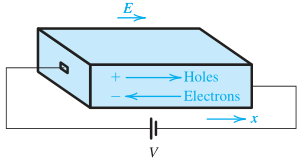
\includegraphics[width=1\textwidth]{img/1/bar-of-silicon.png}
    \end{minipage}
    \hfill
    \begin{minipage}{0.60\textwidth}
        \caption{``An electric field E established in a bar of silicon causes the holes to drift in the direction of E and the free electrons to drift in the opposite direction. Both the hole and electron drift currents are in the direction of E.''\cite{sedra-smith:microelectronic-circuits}}
    \end{minipage}
    \label{fig:bar-of-silicon}
\end{figure}

\renewcommand*{\thefootnote}{\fnsymbol{footnote}}
\footnotetext[4]{%
    À medida que a temperatura aumenta, mais ligações covalentes se rompem, o que resulta em mais pares eletrão-lacuna, aumentando a condutividade do silício.
}
\renewcommand*{\thefootnote}{\arabic{footnote}}

%//==============================--@--==============================//%
\subsection[1.2 Fluxo de corrente nos semicondutores]{\hspace*{0.075 em}\raisebox{0.2 em}{$\pmb{\drsh}$} Fluxo de corrente nos semicondutores}
\label{subsec:current-flow-semiconductors}

O fluxo de corrente nos semicondutores pode ser dividido em dois componentes principais: corrente de deriva e corrente de difusão.

\begin{itemize}[leftmargin=*]
    \item \textbf{Corrente de deriva}:
    \begin{itemize}
        \item[$($\textbf{?}$)$] Causada pelo movimento de portadores de carga (eletrões e lacunas) sob a influência de um campo elétrico externo.
        \item[$\blacktriangle$] A densidade de corrente de deriva, $J_{\textit{drift}}$, pode ser descrita pela fórmula:
        \begin{equation*}
            J_{\textit{drift}} = q(n \mu_n + p \mu_p)E
        \end{equation*}
        onde $q$ é a carga elementar, $n$ e $p$ são as concentrações de eletrões e lacunas (respetivamente), $\mu_n$ e $\mu_p$ são as mobilidades dos eletrões e lacunas, e $E$ é a intensidade do campo elétrico aplicado.
    \end{itemize}

    \item \textbf{Corrente de difusão}:
    \begin{itemize}
        \item[$($\textbf{?}$)$] Causada pelo movimento de portadores de carga devido a gradientes de concentração, ou seja, os portadores de carga movem-se de regiões de maior concentração para regiões de menor concentração.
        \item[$\blacktriangle$] A densidade de corrente de difusão para eletrões, $J_{n, \textit{diff}}$, e lacunas, $J_{p, \textit{diff}}$, pode ser descrita pelas fórmulas:
            \begin{align*}
                J_{n, \textit{diff}} &= -qD_n\frac{dn}{dx} \\
                J_{p, \textit{diff}} &= qD_p\frac{dp}{dx}
            \end{align*}
        onde $D_n$ e $D_p$ são os coeficientes de difusão para eletrões e lacunas, e $dn/dx$ e $dp/dx$ são os gradientes de concentração para eletrões e lacunas, respetivamente.
    \end{itemize}

    \item \textbf{Relação de Einstein}:
    \begin{itemize}
        \item[$($\textbf{?}$)$] Estabelece uma ligação entre o coeficiente de difusão e a mobilidade dos portadores de carga num semicondutor.
        \item[$\blacktriangle$] A relação para eletrões ($D_n$) e lacunas ($D_p$) é dada pelas fórmulas:
            \begin{align*}
                D_n &= \mu_n \frac{k T}{q} \\
                D_p &= \mu_p \frac{k T}{q}
            \end{align*}
        onde $k$ é a constante de Boltzmann, $T$ a temperatura absoluta em Kelvin e $q$ o valor da carga elementar.
        \item[$\blacktriangle$] Esta relação liga os processos de deriva e difusão dos semicondutores, uma vez que implica que o coeficiente de difusão é diretamente proporcional à mobilidade dos portadores de carga. É possível representar a relação sucintamente:
            $$
                \boxed{ \frac{D_n}{\mu_n} = \frac{D_p}{\mu_p} = V_T }
            $$
        onde $V_T \delequal kT/q$. O parâmetro $V_T$ é conhecido como a \textbf{tensão térmica}. 
        
        \textbf{Nota:} À temperatura ambiente, $T \simeq 300$K e $V_T \simeq 25$ mV.    
    \end{itemize}
\end{itemize}
    
%//==============================--@--==============================//%
\clearpage
\subsection[1.3 Junção pn]{\hspace*{0.075 em}\raisebox{0.2 em}{$\pmb{\drsh}$} Junção pn}
\label{subsec:pn-junction}

Uma junção pn é formada quando um semicondutor tipo p (com um excesso de lacunas) é colocado em contacto com um semicondutor tipo n (com um excesso de elétrões).

\begin{figure}[H]
    \centering
    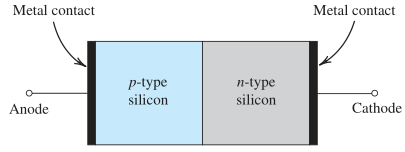
\includegraphics{img/1/simplified-pn-junction.png}
    \caption{``Simplified physical structure of the pn junction. (...)''\cite{sedra-smith:microelectronic-circuits}}
    \label{fig:simplified-pn-junction}
\end{figure}

\begin{figure}[ht] 
    \begin{subfigure}[b]{0.5\linewidth}
        \centering
        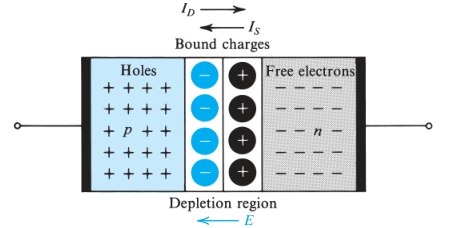
\includegraphics[width=1\linewidth]{img/1/pn-junction-OC.png}
        \caption{} 
        \label{fig:pn-junction-OC} 
    \end{subfigure}%% 
    \begin{subfigure}[b]{0.5\linewidth}
        \centering
        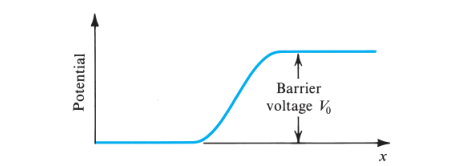
\includegraphics[width=1\linewidth]{img/1/pn-junction-potential-distrib.png} 
        \caption{} 
        \label{fig:pn-junction-potential-distrib} 
    \end{subfigure}  
    \caption{``(a) The pn junction with no applied voltage (open-circuited terminals). (b) The potential distribution along an axis perpendicular to the junction.''\cite{sedra-smith:microelectronic-circuits}}
    \label{fig:pn-junction}
\end{figure}

\vspace{-1em}
\begin{itemize}[leftmargin=*, noitemsep]
    \item \textbf{Corrente de Difusão ($I_D$):}
    \begin{itemize}[leftmargin=*, label=$\pmb{-}$]
        \item Devido à alta concentração de lacunas na região p e baixa concentração na região n, as lacunas difundem-se através da junção do lado p para o lado n.
        \item De maneira semelhante, os eletrões difundem-se através da junção do lado n para o lado p devido à sua alta concentração na região n e baixa concentração na região p.
        \item Estes dois componentes da corrente juntam-se para formar a corrente de difusão $I_D$, que flui do lado p para o lado n.
    \end{itemize}
    
    \item \textbf{Corrente de Deriva/Corrente de Saturação Inversa ($I_S$):}
    \begin{itemize}[leftmargin=*, label=$\pmb{-}$]
        \item Além de $I_D$, existe uma componente da corrente proveniente da deriva de portadores minoritários (\textit{minor carriers}) através da junção.
        \item As lacunas geradas termicamente na região n movem-se em direção à junção, e à beira da região de depleção, são influenciadas pelo campo elétrico, que as arrasta para o lado p.
        \item De maneira semelhante, os eletrões gerados termicamente na região p movem-se para a beira da região de depleção e são arrastados pelo campo elétrico para o lado n.
        \item Estes dois componentes da corrente---eletrões movidos por deriva de p para n e lacunas movidas por deriva de n para p---somam-se para formar a corrente de deriva $I_S$, que flui do lado n para o lado p da junção.
        \item A corrente de deriva $I_S$ é fortemente dependente da temperatura mas independente da tensão da região de depleção $V_0$ $[$que veremos em seguida$]$.
    \end{itemize}
\end{itemize}

\newpage
\begin{itemize}[leftmargin=*, nolistsep]
    \item \textbf{Depletion region:}
    \begin{itemize}[label=$\blacktriangle$, leftmargin=*]
        \item Quando uma junção pn é formada, eletrões da região do tipo n (com excesso de eletrões) difundem-se na região do tipo p (com excesso de lacunas) devido ao gradiente de concentração (\hyperref[subsec:current-flow-semiconductors]{rever fluxo de corrente nos semicondutores}).
        \item Estes eletrões recombinam-se com as lacunas disponíveis na região do tipo p, criando uma região em torno da junção onde os portadores de carga móveis estão reduzidos. Essa região é chamada de \underline{região de depleção} ou \underline{camada de depleção}.
        \item A região de depleção tem uma largura que depende da concentração de dopagem de ambos os materiais do tipo p e do tipo n e da tensão aplicada através da junção. Atua como uma barreira ao fluxo de portadores de carga através da junção sob polarização inversa (\textit{reverse bias}).
    \end{itemize}

    \item \textbf{Built-in potential:}
    \begin{itemize}[label=$\blacktriangle$, leftmargin=*]
    \item À medida que os eletrões se difundem através da junção e se recombinam com as lacunas, deixam para trás iões doadores positivamente carregados na região do tipo n e iões aceitadores negativamente carregados na região do tipo p.
    \item Estes átomos doadores e aceitadores, ionizados e imóveis, criam um campo elétrico que se opõe à difusão adicional dos portadores de carga, impedindo a neutralização completa das impurezas de dopagem.
    \item A diferença de potencial gerada por este campo elétrico é chamada de \textit{built-in potential}. Esta tensão atua como uma barreira que deve ser superada por uma tensão externa para que os portadores de carga atravessem a junção em polarização direta (\textit{forward bias}). 
    
    A \textbf{barrier voltage} pode ser dada por (``$[$with$]$ no external voltage applied $[$...$]$''\cite{sedra-smith:microelectronic-circuits}):
    $$
        V_0 = V_T\, \ln\left(\frac{N_A N_D}{n^{2}_{i}}\right)
    $$
    onde $N_A$ e $N_D$ são as concentrações de dopagem do lado p e do lado n da junção (respetivamente); e $n^{2}_{i} \delequal$ produto da concentração de lacunas e de eletrões livres.
    \end{itemize}

    \item \textbf{Forward bias and reverse bias:}
    \begin{itemize}[label=$\blacktriangle$, leftmargin=*]
        \item O comportamento de uma junção pn depende da polaridade da tensão externa aplicada. Há duas condições: polarização direta e polarização reversa.
        \begin{itemize}[label=\rule{1ex}{1ex}, leftmargin=*]
            \item \textbf{Forward bias (polarização direta):}
            \begin{itemize}[label=$\pmb{-}$]
                \item Na polarização direta, a região do tipo p é conectada ao terminal positivo, e a região do tipo n é conectada ao terminal negativo da fonte de tensão.
                \item Esta tensão externa reduz a barreira de potencial criada pelo \textit{built-in potential}, permitindo que os portadores de carga (lacunas da região do tipo p e eletrões da região do tipo n) atravessem a junção.
                \item A corrente aumenta rapidamente com a tensão aplicada, resultando num fluxo de corrente unidirecional.
            \end{itemize}
        \end{itemize}
        
        \begin{itemize}[label=\rule{1ex}{1ex}, leftmargin=*]
            \item \textbf{Reverse bias (polarização inversa):}
            \begin{itemize}[label=$\pmb{-}$]
                \item Na polarização inversa, a região do tipo p é conectada ao terminal negativo, e a região do tipo n é conectada ao terminal positivo da fonte de tensão.
                \item Esta tensão externa aumenta a barreira de potencial, impedindo o fluxo de portadores de carga através da junção.
                \item A corrente é insignificante, tipicamente limitada a uma pequena corrente de saturação inversa devido à presença de portadores minoritários e portadores gerados termicamente.
            \end{itemize}
        \end{itemize}
    \end{itemize}
\end{itemize}

%//==============================--@--==============================//%
    
    \clearpage
    \section{2. Díodos e retificadores}\label{sec:diodes-and-rectifiers}%
        %//==============================--@--==============================//%

\noindent O díodo é um dispositivo eletrónico de dois terminais que pode ser utilizado como elemento básico não-linear para realizar circuitos variados com especial incidência nos conversores de potência que transformam a tensão alternada da rede de distribuição de energia elétrica nas tensões contínuas necessárias para a alimentação de diversos equipamentos de cariz eletrónico.

%//==============================--@--==============================//%
\subsection[2.1 Díodos de junção]{\hspace*{0.075 em}\raisebox{0.2 em}{$\pmb{\drsh}$} Díodos de junção}
\label{subsec:junction-diode}
\noindent O díodo possui dois terminais, ânodo e cátodo, provenientes do contacto metálico entre os dois semicondutores. O sentido ilustrado é o de $p$ para $n$. Designaremos por $i_D$ a corrente e por $v_D$ a tensão que atravessam o díodo.

\begin{figure}[H]
    \centering
    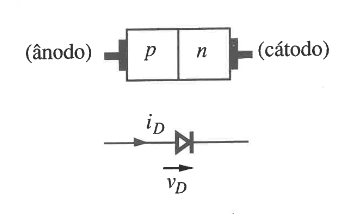
\includegraphics[width = 0.45\linewidth]{img/2/diode.png}
    \caption{Díodo de junção.}
    \label{fig:diode}
\end{figure}

\noindent A característica do díodo, isto é, a relação entre a corrente e a tensão $i_D(v_D)$ pode ser seccionada em 3 zonas de operação, mediante a polarização aplicada\footnotemark:

\vspace{-0.5 em}
\begin{figure}[H]
    \centering
    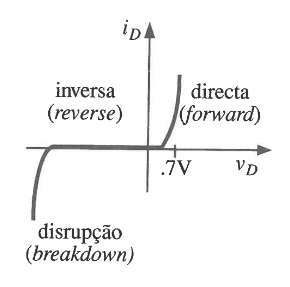
\includegraphics[width = 0.4\linewidth]{img/2/curve.png}
    \caption{Característica do díodo de junção.}
    \label{fig:curve}
\end{figure}

\begin{itemize}
    \item \textbf{Zona de disrupção:} $v_D < 0$ e $v_D$ excede um valor específico de forma a que $i_D < 0$. Possui um comportamento indesejável com exceção nos díodos de Zener, que operam exclusivamente nesta zona.
    \item \textbf{Zona inversa:} $v_D < 0$ e $i_D = 0$. O circuito diz-se cortado.
    \item \textbf{Zona direta:} $v_D > 0$ e $i_D > 0$. O circuito conduz.
    \end{itemize}

%---footnote---%
\footnotetext{Quando $v_D > 0$ diz-se que o díodo possui polarização direta e quando $v_D < 0$ diz-se que possui polarização inversa.}
%---footnote---%

\newpage
\noindent A curva característica possui a seguinte fórmula:
$$
    \boxed{i_D = I_s(e^{v_D/nV_T} - 1)}
$$
\begin{itemize}
    \item[$\pmb{I_s \rightarrow}$] Corrente inversa de saturação. Proporcional à área de junção $pn$.
    \item[$\pmb{V_T \rightarrow}$] Tensão térmica. $V_T = k T/ q$ onde $k$ é a constante de Boltzman, $T$ a temperatura absoluta (tipicamente $T = 300$K) e $q$ a carga do eletrão (\hyperref[subsec:current-flow-semiconductors]{como definido acima}).
    \item[$\pmb{n \rightarrow}$] Coeficiente dependente do material e dimensão do díodo. $1 < n < 2$ onde $n = 2$ quando o díodo é considerado como um componente discreto e $n \simeq 1$ enquanto componente integrado.
\end{itemize}

\noindent\textbf{Nota:} Normalmente $v_D \gg n V_T$ e portanto é considerada a seguinte aproximação:
$$
    \boxed{i_D \simeq I_s e^{v_D/nV_T}}
$$
Mediante esta fórmula podemos tomar as seguintes aproximaçãos:
\begin{itemize}
    \item O díodo permanece cortado para $v_D < 0.5$V.
    \item O díodo conduz para $v_D > 0.7$V.
\end{itemize}

%//==============================--@--==============================//%
\subsubsection[2.1.1 Aproximação linear por troço]{$\pmb{\rightarrow}$ Aproximação linear por troço}

\noindent Assim, é fácil estabelecer uma \textbf{aproximação linear por troço} da característica dos díodos. Com um grau crescente de complexidade (e, consequentemente de rigor) podem considerar-se as três formas de aproximação:

\vspace{0.5 em}
\begin{center}
    \begin{minipage}{0.6\textwidth}
        \begin{itemize}[leftmargin=*]
        \item[] \textbf{\emph{Díodo ideal}}: Num circuito em que o nível de tensões é $\gg v_D = 0.7$V podemos desprezar $v_D$. Desta forma, para $v_D < 0$, $i_D = 0$ e para $i_D > 0$, $v_D = 0$. O díodo é equivalente a um circuito aberto na primeira instância e a um curto circuito na segunda. 
        \end{itemize}
    \end{minipage}%
    \hfill
    \begin{minipage}{0.4\textwidth}
        \begin{center}
            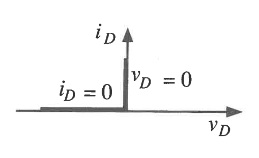
\includegraphics[width=0.9\textwidth]{img/2/ideal.png}
            \label{img:ideal}
        \end{center}
    \end{minipage}
\end{center}

\begin{center}
    \begin{minipage}{0.6\textwidth}
        \begin{itemize}[leftmargin=*]
        \item[] \textbf{\emph{Díodo com tensão constante}}: Admite-se que quando o díodo conduz $v_D = 0.7$V, sendo $i_D = 0$ para $v_D < 0$. O díodo é representado pelo esquema equivalente da \hyperref[fig:tensao-const-esquema]{Fig.\;4 (a)}, constituído por um díodo ideal em série com um gerador de tensão de $V_D = 0.7$V.
        \end{itemize}
    \end{minipage}%
    \hfill
    \begin{minipage}{0.4\textwidth}
        \begin{center}
            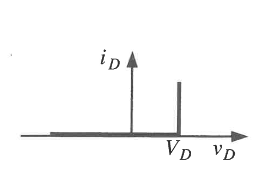
\includegraphics[width=0.9\textwidth]{img/2/tensao-const.png}
            \label{img:tesao-const}
        \end{center}
    \end{minipage}
\end{center}

\begin{center}
    \begin{minipage}{0.6\textwidth}
        \begin{itemize}[leftmargin=*]
        \item[] \textbf{\emph{Díodo com resistência incremental}}: A carac- terística passa a ser aproximada por dois troços de reta. O esquema equivalente (\hyperref[fig:resi-esquema]{Fig.\;4 (b)}) passa a ser constituído por um díodo ideal em série com um gerador de tensão, $V_{D0} \ge 0.5$V, e com resistência incremental, correspondente ao inverso da inclinação da característica: $\Delta v_D/ \Delta i_D$.
        \end{itemize}
    \end{minipage}%
    \hfill
    \begin{minipage}{0.4\textwidth}
        \begin{center}
            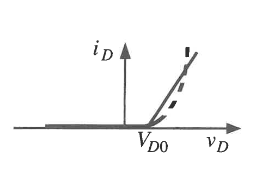
\includegraphics[width=0.9\textwidth]{img/2/resis.png}
            \label{img:resis}
        \end{center}
    \end{minipage}
\end{center}

\begin{figure}[ht] 
    \begin{subfigure}[b]{0.5\linewidth}
        \centering
        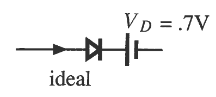
\includegraphics[width=0.5\linewidth]{img/2/tensao-const--esquema.png}
        \caption{Esquema equivalente para o modelo de tensão constante.} 
        \label{fig:tensao-const-esquema} 
        \vspace{1ex}
    \end{subfigure}%% 
    \begin{subfigure}[b]{0.5\linewidth}
        \centering
        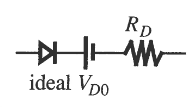
\includegraphics[width=0.5\linewidth]{img/2/resi-esquema.png} 
        \caption{Esquema equivalente para o modelo de resistência.} 
        \label{fig:resi-esquema} 
        \vspace{1ex}
    \end{subfigure} 
    \caption{Esquemas equivalentes das aproximações lineares por troço.}
    \label{fig:esquema}
\end{figure}

%//==============================--@--==============================//%
\subsubsection[2.1.2 Rede resistiva com um só díodo]{$\pmb{\rightarrow}$ Rede resistiva com um só díodo}

\noindent A análise de uma rede resistiva com um só díodo, pode fazer-se com relativa facilidade se se usar o teorema de Thévenin se substituir a rede “vista” pelo díodo pelo seu esquema equivalente de aproximação linear. As variáveis $v_D$, e $i_D$, têm que satisfazer a característica do díodo e têm também que satisfazer a equação que resulta da lei das tensões aplicada ao circuito:

\vspace{-1 em}
\begin{figure}[H]
    \centering
    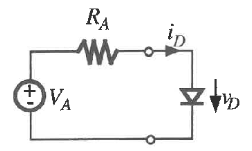
\includegraphics[width = 0.45\linewidth]{img/2/resi-diode-net.png}
    \caption{Rede resistiva com um só díodo.}
    \label{fig:resi-diode-net}
\end{figure}

\vspace{-1 em}
$$
    \boxed{V_A = R_A i_D + v_D}
$$

\paragraph[2.1.2.1 Reta de Carga]{$\pmb{\star}$ Reta de carga}\mbox{}\\[4pt]
\noindent $V_D$ e $I_D$ podem ser determinados fazendo uso de um \textbf{método gráfico}:

\vspace{-1.25 em}
\begin{figure}[H]
    \centering
    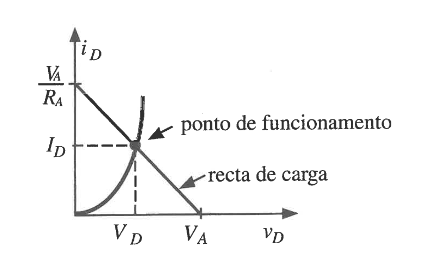
\includegraphics[width = 0.5\linewidth]{img/2/reta-carga.png}
    \caption{Método gráfico: reta de carga.}
    \label{fig:reta-carga}
\end{figure}

\noindent A \textbf{reta de carga} pode ser facilmente traçada através da interseção com os eixos:
$$
    \left.
    \begin{aligned}
        v_D = V_A\quad &\text{e}\quad i_D = 0  \\
        v_D = 0\quad   &\text{e}\quad i_D = V_A/R_A 
    \end{aligned} 
    \;\right\}
    \mkern12mu \begin{minipage}{0.6\textwidth}
                    O \underline{ponto de funcionamento}, oriundo da interseção da reta com a curva característica do díodo, possui as coordenadas de $I_D$ e $V_D$.
              \end{minipage}
$$

\newpage
\paragraph[2.1.2.2 Método iterativo]{$\pmb{\star}$ Método iterativo}\mbox{}\\[4pt]
A análise do circuito pode também ser realizada com recurso a um método iterativo. Invertendo a equação da curva característica simplificada do díodo obtemos:
$$
    v_D \simeq n V_T \ln(i_D/I_s)
$$
Recorrendo a dois possíveis pontos de coordenadas $(v_{DX}, i_{DX})$ e  $(v_{DY}, i_{DY})$ obtemos a seguinte relação:

\vspace{-2em}
\begin{align*}
    v_{DY} &\simeq v_{DX} + n V_T \ln(i_{DY}/i_{DX}) \\
    i_{DY} &= (V_A - V_{DX})/R_A
\end{align*}

\noindent Para aplicar o método iterativo parte-se de uma estimativa $i_{D0}$ e admite-se que a tensão correspondente é $0.7$V. A partir daí aplica-se as duas equações supramencionadas alternadamente:
\begin{empheq}[box=\widefbox]{align*}
        i_{D0} &= \textbf{estimativa}\\
        v_{DY} &= 0.7\text{V}\\
        i_{D1} &= (V_A - V_{D0})/R_A\\
        v_{D1} &\simeq v_{D0} + n V_T \ln{(i_{D1}/i_{D0})}\\
        i_{D2} &= (V_A - V_{D1})/R_A\\
        v_{D2} &\simeq v_{D1} + n V_T \ln{(i_{D2}/i_{D1})}\\
        &\mkern64mu \pmb{\cdots}
\end{empheq}

%//==============================--@--==============================//%
\subsection[2.2 Díodo Zener]{\hspace*{0.075 em}\raisebox{0.2 em}{$\pmb{\drsh}$} Díodo Zener}
\label{subsec:zener-diode}

A íngreme curva $i-v$ destes díodos na \textit{breakdown region} (\hyperref[fig:zener-diode]{Fig. 9 (a)}), indica uma queda de tensão quase constante\footnotemark[2]---algo que sugere o seu uso em reguladores de tensão.

\vspace{-0.5em}
\begin{figure}[H]
    \begin{subfigure}{0.5\textwidth}
        \centering
        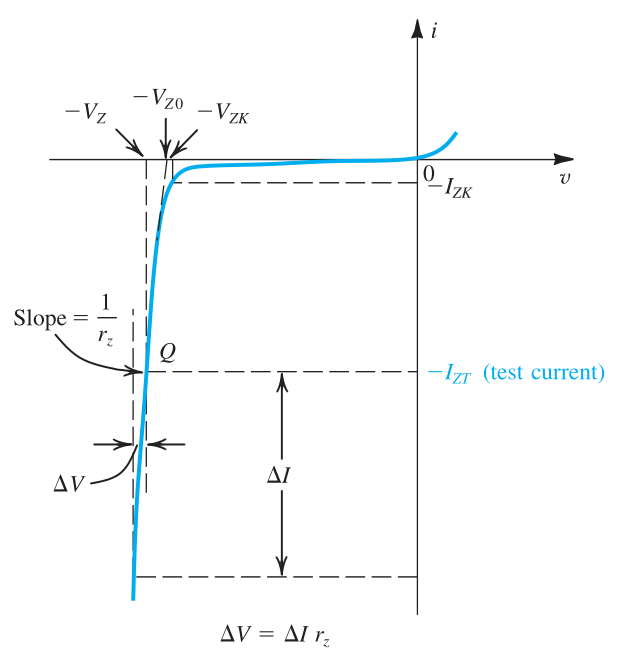
\includegraphics[width=\linewidth]{img/2/zener-diode-iv.png}
        \caption{``The diode i–v characteristic (...)''\cite{sedra-smith:microelectronic-circuits}}
    \end{subfigure}
    \begin{subfigure}{0.45\textwidth}
        \centering
        \raisebox{10.78em}{
            \begin{minipage}{\textwidth}
                \begin{minipage}{\textwidth}
                    \centering
                    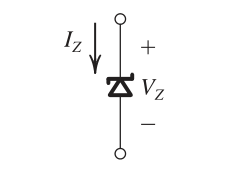
\includegraphics[width=0.6\linewidth]{img/2/zener-diode.png}
                    \caption{``Circuit symbol for a zener diode.''\cite{sedra-smith:microelectronic-circuits}}
                \end{minipage}
                \begin{minipage}{\textwidth}
                    \centering
                    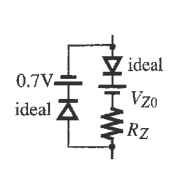
\includegraphics[width=0.45\linewidth]{img/2/zener-diode-model.png}
                    $$
                        \boxed{ V_Z = V_{Z0} + r_Z I_Z }
                    $$
                    \caption{``Esquema equivalente com resistência.''\cite{medeiros:ICEE}}
                \end{minipage}
            \end{minipage}
        }
    \end{subfigure}
    \caption{Díodo Zener: conhecidos como díodos de rutura ou zener; normalmente têm o cátodo positivo (com a corrente a fluir para este), o que resulta em \underline{valores positivos para $I_Z$ e $V_Z$} na prática, como indica o esquema equivalente (c).}
    \label{fig:zener-diode}
\end{figure}

\footnotetext[2]{%
    Para correntes superiores à corrente de joelho (\textit{knee current}) $I_{ZK}$, a característica $i-v$ do diodo zener é quase linear. O fabricante normalmente especifica a tensão $V_Z$ num dado $I_{ZT}$ (a corrente de teste).
}
%//==============================--@--==============================//%
        \clearpage
%//==============================--@--==============================//%
\subsection[2.2 Retificadores]{\hspace*{0.075 em}\raisebox{0.2 em}{$\pmb{\drsh}$} Retificadores}
\label{subsec:rectifiers}

\noindent Os retificadores constituem a aplicação mais simples e mais frequente dos díodos. Existem dois tipos de retificadores: os retificadores de meia onda e os retificadores de onda completa.

%//==============================--@--==============================//%
\subsubsection[2.2.1 Retificadores de meia onda]{$\pmb{\rightarrow}$ Retificadores de meia onda}

\vspace{-1 em}
\begin{figure}[H]
    \centering
    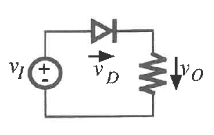
\includegraphics[width = 0.4\linewidth]{img/2/ret-meia-onda.png}
    \caption{retificador de meia onda com díodo ideal}
    \label{fig:ret-meia-onda}
\end{figure}

\noindent Supondo que a tensão no díodo, quando este conduz, não é desprezável,
utilizamos a aproximação linear por troços, nomeadamente o modelo de resistência incremental:

\begin{itemize}[leftmargin=*]
    \item Se $v_I < V_{D0}$, $v_D < 0$ e consequentemente $i_D = 0$. Díodo ideal como circuito aberto.
    \item Se $v_I > V_{D0}$, $v_D = 0$ e consequentemente $i_D > 0$. Díodo ideal equivalente a um curto circuito. Operando sobre a malha do circuito $v_o = \frac{R}{R + R_D}(v_I - V_{D0})$. Se $R_D \ll R$ fica a aproximação $v_O \simeq v_I - V_{D0}$.
\end{itemize}

\noindent No caso de $v_I$ ser uma sinusoide simplesmente retificada, tem interesse determinar o seu valor médio:
$$
    \boxed{(v_O)_{\textit{avg}} = \frac{1}{T} \int_{0}^{T} v_O(t) \, dt = \dfrac{V_m}{\pi}}
$$
\begin{mdframed}
\begin{itemize}[leftmargin=*, nolistsep]
    \item \textbf{\underline{Nota:} Dimensionamento de um díodo}
    \begin{itemize}[leftmargin=*]
    \item Dois parâmetros importantes a especificar:
        \begin{enumerate}
        \item \textbf{Capacidade de manuseio da corrente}: determinada pela maior corrente que se espera que o díodo conduza.
        \item \textbf{Tensão inversa máxima}: o díodo deve ser capaz de suportar este valor sem ocorrer disrupção (\textit{breakdown}); determinado pela maior tensão inversa esperada no díodo.
        \end{enumerate}
    \end{itemize}
\end{itemize}
\end{mdframed}

\noindent A \textbf{capacidade de manuseio da corrente} é calculada com o díodo em \textbf{curto circuito}:
$$
    \boxed{(i_D)_\textit{max} = V_m/R}
$$
\noindent A \textbf{tensão inversa máxima} é calculada com o díodo em \textbf{circuito aberto}, para o circuito em questão é dada por:
$$
    \boxed{(-v_D)_\textit{max} = V_m}
$$

\vspace{-1 em}
\begin{figure}[H]
    \centering
    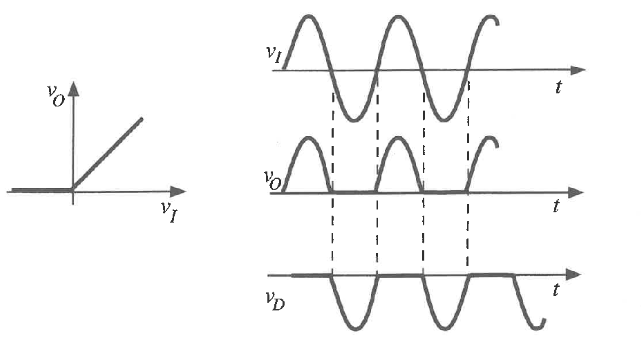
\includegraphics[width = 0.8\linewidth]{img/2/ret-curve.png}
    \caption{Curva da característica $v_O(v_I)$ e respetivo output}
    \label{fig:ret-curve}
\end{figure}

\begin{quote}
    ``Um rectificador transforma uma tensão \textbf{alternada} (com valores positivos e negativos) numa tensão \textbf{unidireccional}''\cite{medeiros:ICEE}
\end{quote}

\noindent Uma das aplicações dos retificadores de meia onda verifica-se na \textbf{desmodulação de amplitude}\footnotemark[3]. Um \textbf{detetor de pico/envolvente} pode ser implementado ao adicionar um \underline{condensador em paralelo} com a resistência de saída.

\footnotetext[3]{``Para tal, é necessário que a constante de tempo $RC$ seja muito maior que o período da sinusoide, para que o condensador não descarregue significativamente entre uma alternância e a seguinte. Por outro lado, é necessário que $RC$ seja menor que o período mínimo do sinal modulante para que $v_O$, possa acompanhar as variações da amplitude da sinusoide.''\cite{medeiros:ICEE}}

Outra aplicação significativa do retificador \underline{com condensador} é como \textbf{conversor corrente alternada/corrente contínua} (AC/DC), em \textbf{fontes de alimentação} (\textit{power supplies}).

\vspace{0.9 em}
\noindent Na realidade, nas aplicações com condensadores, a tensão de saída apresenta uma componente variável (induzida pela carga/descarga do condensador) designada por \textbf{tremor} ou \textbf{ondulação} (\textit{ripple}).

\begin{quote}
    ``Pode fazer-se uma \underline{estimativa da amplitude do tremor}, $\Delta v_O$. A carga perdida pelo condensador durante a maior parte do período,
    $$
        \Delta Q \approx I\, \Delta t = \frac{V_m}{R}\, T
    $$
    é igual a carga reposta no condensador quando o díodo conduz, durante um breve intervalo de tempo, na vizinhança do máximo de $v_I(t)$
    $$
        \Delta Q \approx C\, \Delta v_O
    $$
    Resulta que o tremor, em valor relativo, é
    $$
        \frac{\Delta v_O}{V_m} \approx \frac{T}{RC}
    $$
    Em vez de um condensador, podem usar-se filtros LC para reduzir o tremor.''\cite{medeiros:ICEE}
\end{quote}

%//==============================--@--==============================//%
\subsubsection[2.2.1 Retificadores de onda completa]{$\pmb{\rightarrow}$ Retificadores de onda completa}

\begin{quote}
    ``The full-wave rectifier utilizes both halves of the input sinusoid. To provide a unipolar output,
    it \underline{inverts the negative halves} of the wave.''\cite{sedra-smith:microelectronic-circuits}
\end{quote}

\begin{figure}[H]
    \centering
    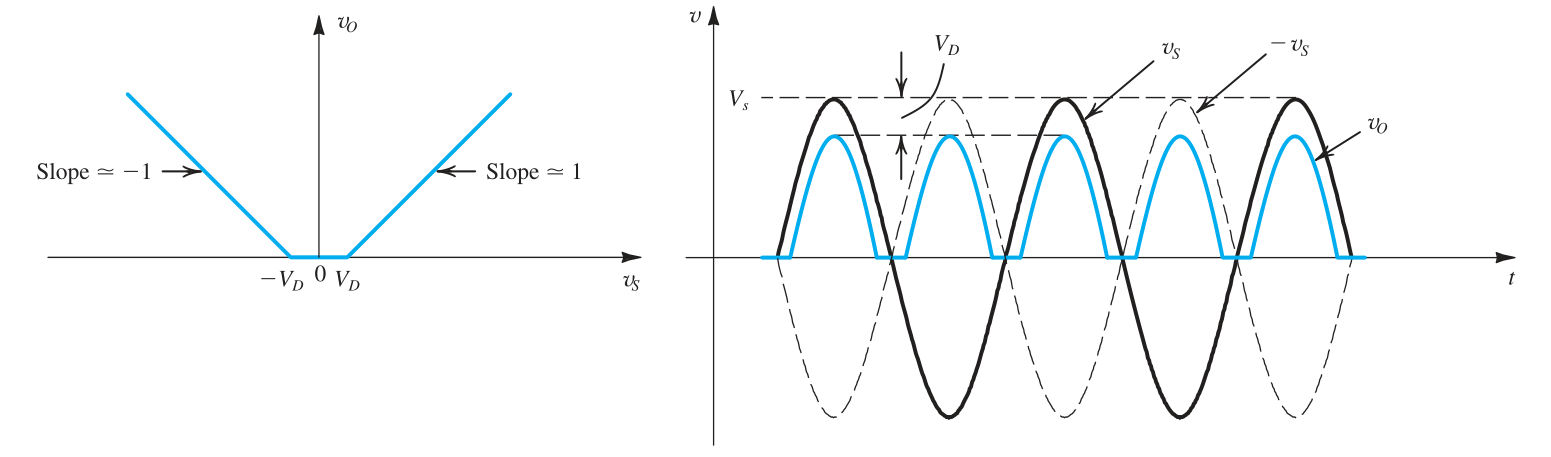
\includegraphics[width=1\linewidth]{img/2/exemplo-full-wave-rectifier.png}
    \caption{``(left) transfer characteristic assuming a constant-voltage-drop model for the diodes; (right) input and output waveforms.''\cite{sedra-smith:microelectronic-circuits}}
    \label{fig:exemplo-full-wave-rectifier}
\end{figure}

%//==============================--@--==============================//%
\paragraph[2.2.1.1 Implementação com um transformador]{$\pmb{\star}$ Implementação com um transformador}\mbox{}

\begin{figure}[H]
    \centering
    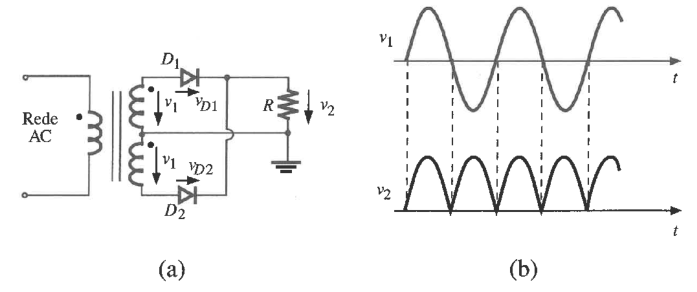
\includegraphics[width = 0.8\linewidth]{img/2/onda-completa-transformador.png}
    \caption{``Rectificador de onda completa com transformador com tomada no ponto médio do secundário.''\cite{medeiros:ICEE}}
    \label{fig:onda-completa-transformador}
\end{figure}

\noindent A ação do retificador de onda completa pode ser descrita da seguinte forma:
\begin{itemize}[leftmargin=*]
    \item Se $v_I < V_{D0}$, $v_{D1} < 0$ e $v_{D2} > 0$, D$_1$ está cortado e D$_2$ conduz. $v_2 = -v_1 - v_D \simeq - v_1$
    \item Se $v_I > V_{D0}$, $v_{D1} > 0$ e $v_{D2} < 0$, D$_2$ está cortado e D$_1$ conduz. $v_2 = v_1 + v_D \simeq  v_1$
    \item Logo $v_2 \simeq |v_1|$
\end{itemize}

\noindent No caso de $v_I$ ser uma sinusoide simplesmente retificada, podemos calcular novamente o seu o seu valor médio:
$$
    \boxed{(v_2)_{\textit{avg}} = \frac{1}{T} \int_{0}^{T} v_O(t) \, dt = \dfrac{2V_m}{\pi}}
$$

\noindent A \textbf{tensão inversa máxima} é calculada com o díodo 1 ou 2 em \textbf{circuito aberto}. Supondo $v_I > V_{D0}$ e o díodo 2 em aberto:
$$
    v_{D2} = -V_I - V_2\; \pmb{\longrightarrow}\; (-v_D)_{\text{máx}} = V_I + V_2
$$
\noindent $V_2$ é máximo para $V_I - V_{D1}$, logo:
$$
    \boxed{(-v_D)_{\text{max}} = 2V_m - V_{D1}}
$$

%//==============================--@--==============================//%
\clearpage
\paragraph[2.2.1.2 Implementação em ponte de Graetz]{$\pmb{\star}$ Implementação em ponte de Graetz (\textit{Bridge Rectifier})}\mbox{}

\begin{quote}
    ``An alternative implementation of the full-wave rectifier is the bridge rectifier. This circuit, is known as the bridge rectifier because of the similarity of its configuration to that of the Wheatstone bridge, does not require a center-tapped transformer, a distinct advantage over the full-wave rectifier circuit"\cite{sedra-smith:microelectronic-circuits}
\end{quote}

\begin{figure}[H]
    \centering
    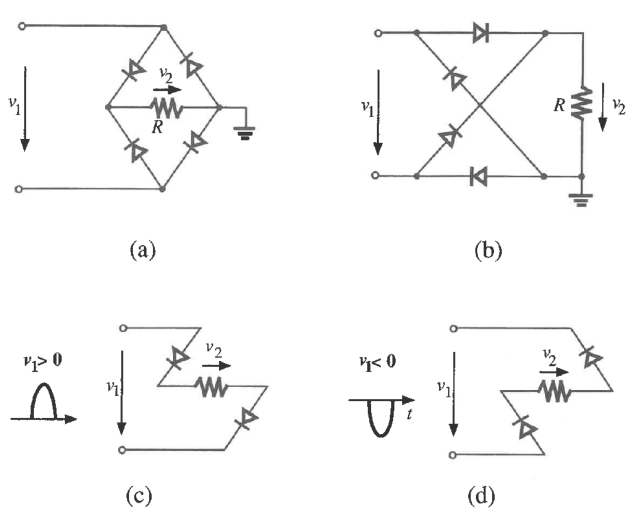
\includegraphics[width = 0.65\linewidth]{img/2/ponte-graetz.png}
    \caption{``Rectificador em ponte de Graetz.''\cite{medeiros:ICEE}}
    \label{fig:ponte-graetz}
\end{figure}

\begin{itemize}
    \item Nas alternâncias positivas de $v_i$, apenas conduzem dois dos díodos, como se indica na \hyperref[fig:ponte-graetz]{Fig. 12 (c)}, obtendo-se:
    $$
        v_2 = v_1 - 2V_D \simeq v_1
    $$
    \item Nas alternâncias negativas de $v_i$, conduzem os díodos contrários, como se indica na \hyperref[fig:ponte-graetz]{Fig. 12 (d)}, obtendo-se:
    $$
        v_2 = - v_1 - 2V_D \simeq  - v_1
    $$
    \item Logo:
    $$
        v_2 \simeq |v_1|
    $$
\end{itemize}

\noindent A \textbf{tensão inversa máxima} é dada por:
$$
    v_{D2} = -V_D - V_2\; \pmb{\longrightarrow}\; (-v_D)_{\text{máx}} = V_D + V_2
$$
\noindent $V_2$ é máximo para $V_m - 2V_{D}$, logo:
$$
    \boxed{(-v_D)_{\text{max}} = V_m - V_{D}}
$$

\noindent Comparando o rectificador em ponte com o circuito anterior, pode concluir-se que o circuito em ponte emprega quatro díodos, em vez de dois, mas tem as seguintes vantagens:

\begin{itemize}
    \item  O transformador é mais simples, uma vez que o secundário não tem tomada central e, para as mesmas tensões, tem metade do número de espiras;
    \item \underline{Tensão inversa máxima} nos díodos é aproximadamente \underline{metade}.
\end{itemize}

%//==============================--@--==============================//%
        \clearpage
%//==============================--@--==============================//%
\subsection[2.3 Reguladores de tensão]{\hspace*{0.075 em}\raisebox{0.2 em}{$\pmb{\drsh}$} Reguladores de tensão}
\label{subsec:reguladores-tensao}

\begin{figure}[H]
    \centering
    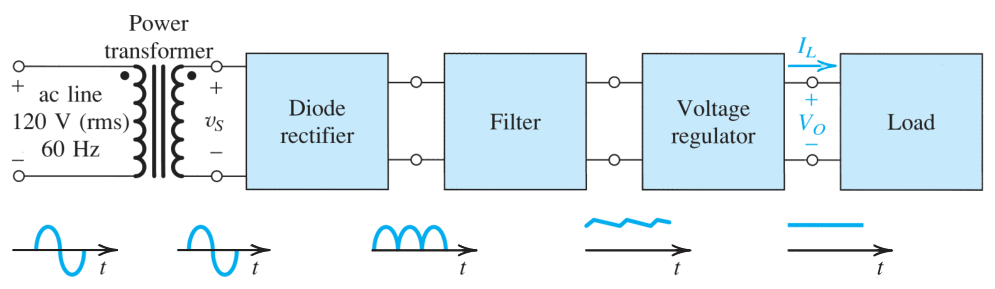
\includegraphics[width=0.8\linewidth]{img/2/power-supply-block-diagram.png}
    \caption{Exemplo com aplicações de díodos. ``Block diagram of a DC power supply.''\cite{sedra-smith:microelectronic-circuits}}
    \label{fig:power-supply-block-diagram}
\end{figure}

\renewcommand*{\thefootnote}{\fnsymbol{footnote}}
\footnotetext[4]{%
    ``Nas fontes de alimentação usa-se, normalmente, um transformador, de modo a baixar a amplitude da tensão alternada e, consequentemente, o valor da tensão continua produzida. Isto é necessário porque a tensão da rede tem amplitude elevada ($220 \sqrt{2} = 311$V) e as tensões contínuas para alimentação dos circuitos electrónicos são muito menores (por exemplo, $12$V). O transformador tem, além disso, a vantagem de produzir \textbf{isolamento galvânico} em relação à rede (há apenas ligação magnética entre os enrolamentos do transformador), o que é útil do ponto de vista da segurança.''\cite{medeiros:ICEE}
}
\renewcommand*{\thefootnote}{\arabic{footnote}}

\noindent Uma \textbf{fonte de tensão} tem como objetivo produzir uma tensão $v_O$ constante. Para tal, necessita, após do retificador e do filtro RC previamente discutido, de um \textbf{regulador de tensão} com vista a \textbf{reduzir o tremor}:

\begin{figure}[H]
    \centering
    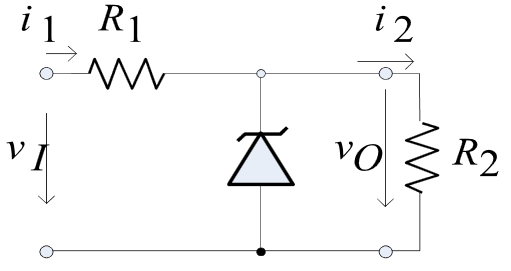
\includegraphics[width = 0.4\linewidth]{img/2/reg-ten.png}
    \caption{Regulador de tensão}
    \label{fig:reg-tensão}
\end{figure}

\begin{quote}
    ``\textbf{Zener Diodes} can be used to produce a \underline{stabilised voltage output} with low ripple under varying load current conditions. By passing a small current through the diode from a voltage source, via a suitable \underline{current limiting resistor} ($R_1$), the zener diode will conduct sufficient current to maintain a voltage drop of $V_\textit{out}$."
\end{quote}

\vspace{0.7 em}
\begin{center}
    \begin{minipage}{0.6\textwidth}
        \begin{itemize}[leftmargin=*]
        \item[] Supondo o díodo em corte:
        $$
            \boxed{v_O = \dfrac{R_2}{R_1 + R_2}v_I}
        $$

        Quando $v_O$ (que se encontra dependente de $v_I$) ultrapassa o treshold $V_Z$ (isto é, $v_I > V_Z$), a tensão na \textit{load} é limitada a $V_Z$. 
        
        Quando $v_O > V_Z$ o díodo entra em condução:
        $$
            \boxed{v_O = V_Z}
        $$
        \end{itemize}
    \end{minipage}%
    \hfill
    \begin{minipage}{0.4\textwidth}
        \begin{center}
            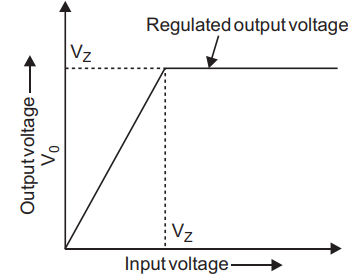
\includegraphics[width=0.9\textwidth]{img/2/chara-ten-reg.png}
            \label{img:chara-ten-reg}
        \end{center}
    \end{minipage}
\end{center}
\noindent \textbf{Nota:} Usa-se para potências muito baixas, de forma a que $i_2 \simeq 0$
%//==============================--@--==============================//%
        \clearpage
%//==============================--@--==============================//%
\subsection[2.4 Limitadores e Fixadores]{\hspace*{0.075 em}\raisebox{0.2 em}{$\pmb{\drsh}$} Limitadores e Fixadores}
\label{subsec:limitadores-e-fixadores}

%//==============================--@--==============================//%
\subsubsection[2.4.1 Limitadores]{$\pmb{\rightarrow}$ Limitadores}

\begin{quote}
    ``O \textbf{limitador} (\textit{clipper}) é um circuito cuja tensão de saída tem um limite superior, um limite inferior, ou ambos os limites, sendo proporcional à tensão de entrada enquanto estes limites não são atingidos.''\cite{medeiros:ICEE}
\end{quote}

\vspace{-1.5em}
\begin{figure}[H]
    \centering
    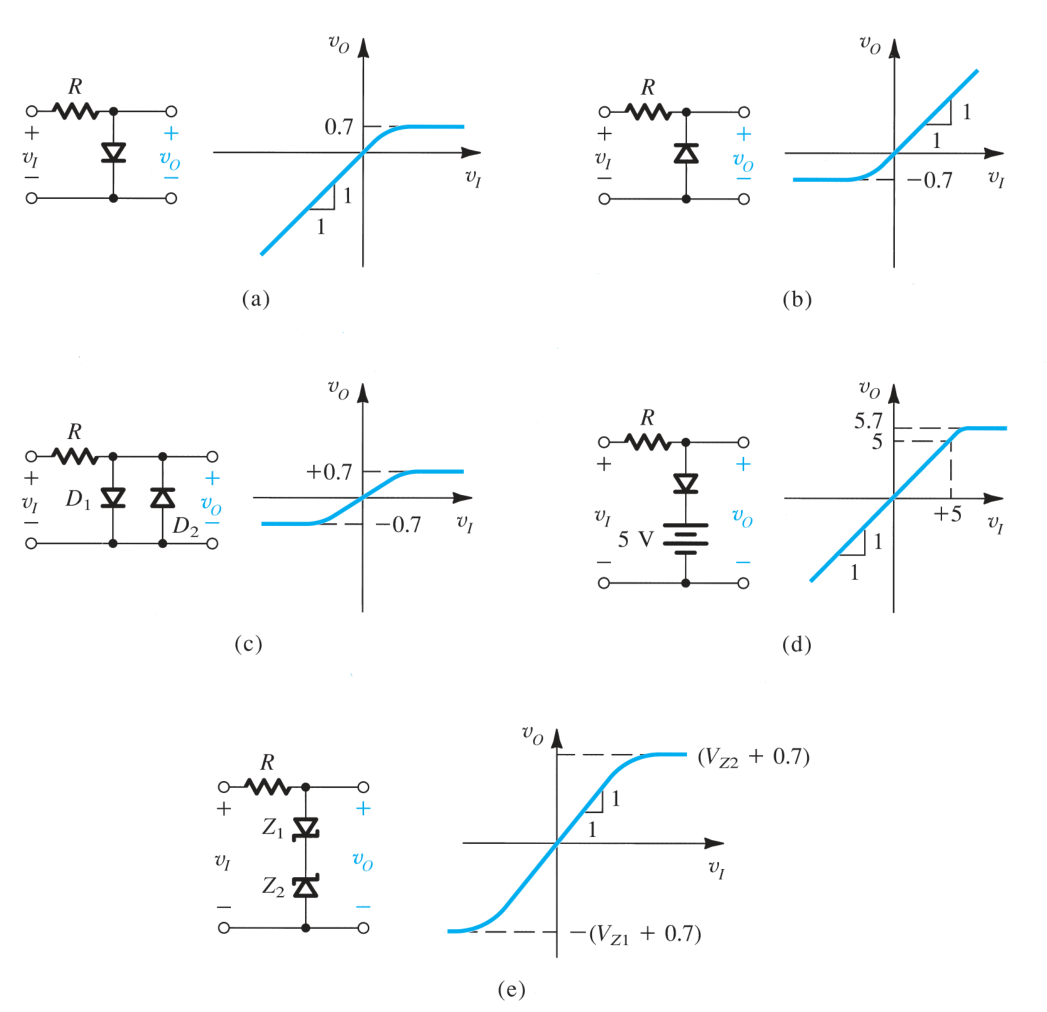
\includegraphics[width=0.8\linewidth]{img/2/limitadores.png}
    \caption{``A variety of basic limiting circuits.''\cite{sedra-smith:microelectronic-circuits}}
    \label{fig:limitadores}
\end{figure}

%//==============================--@--==============================//%
\subsubsection[2.4.2 Fixadores]{$\pmb{\rightarrow}$ Fixadores}

\begin{quote}
    ``O \textbf{fixador} (\textit{clamper}) é um circuito cuja tensão de saída tem a mesma forma que a tensão de entrada, mas em que o seu valor minimo, ou o seu valor máximo, é fixo e independente da tensão de entrada.''\cite{medeiros:ICEE}
\end{quote}

\vspace{-1.5em}
\begin{figure}[H]
    \centering
    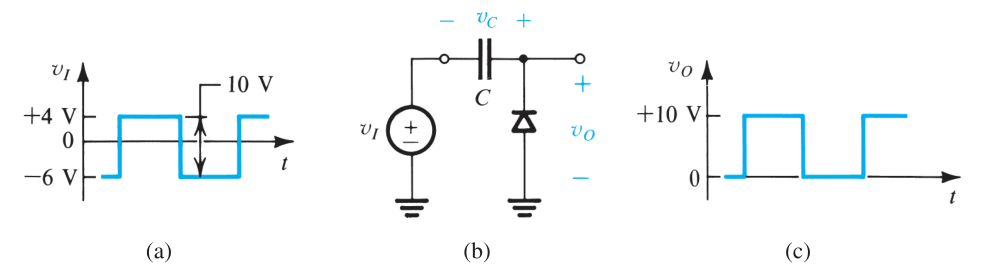
\includegraphics[width=0.85\linewidth]{img/2/fixador.png}
    \caption{``The \textbf{clamped capacitor} or \textbf{dc restorer} with a square-wave input and no load. Because of the polarity in which the diode is connected, the capacitor will charge to a voltage $v_C$ with the polarity indicated and equal to the magnitude of the most negative peak of the input signal. Subsequently, the diode turns off and the capacitor retains its voltage indefinitely.''\cite{sedra-smith:microelectronic-circuits}}
    \label{fig:fixador}
\end{figure}
%//==============================--@--==============================//%

    \clearpage
    \section{3. Circuitos Básicos Analógicos}\label{sec:transistors-BJT-MOS}%
        %//==============================--@--==============================//%
\subsection[3.1 Transístor de junção bipolar (BJT)]{\hspace*{0.075 em}\raisebox{0.2 em}{$\pmb{\drsh}$} Transístor de junção bipolar (BJT)}
\label{subsec:transístor-BJT}

O \textbf{transístor de junção bipolar} ou \textbf{transístor bipolar} (BJT) pode ser visto como um dispositivo de três terminais, descrito em termos das suas correntes e tensões; a designação de "bipolar" resulta da intervenção de cargas negativas (eletrões) e positivas (lacunas) no seu funcionamento (em contraste com os MOSFET que veremos mais adiante).

\begin{figure}[H]
    \centering
    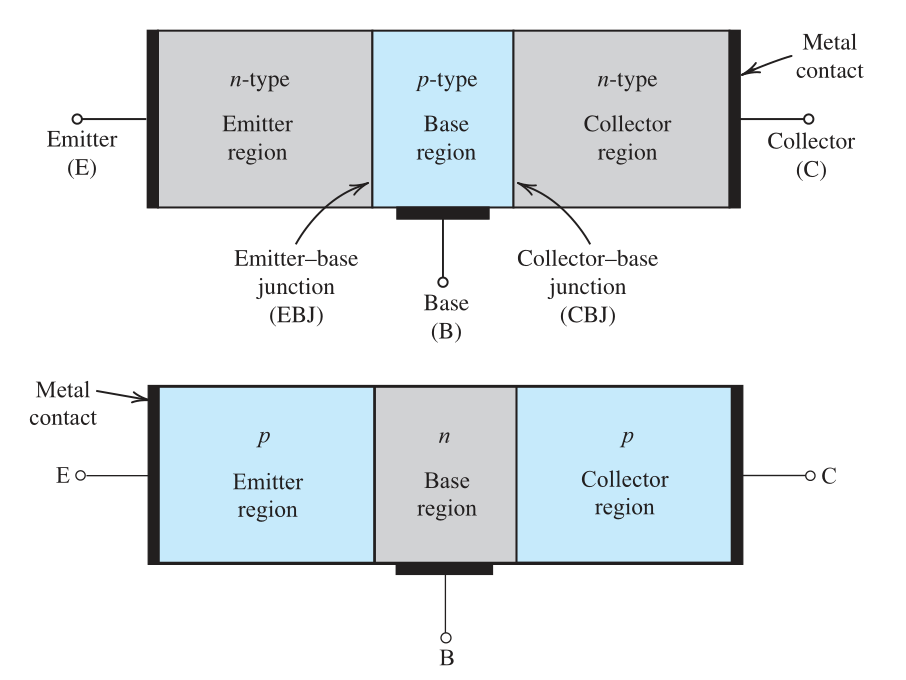
\includegraphics[width=0.7\linewidth]{img/3/BJT/npn-pnp-structure.png}
    \caption{``A simplified structure of the \textit{npn}/\textit{pnp} transistor.''\cite{sedra-smith:microelectronic-circuits}}
    \label{fig:npn-pnp-structure}
\end{figure}

\begin{itemize}[leftmargin=*]
    \item \textbf{Estrutura simplificada do BJT:} Um transístor bipolar consiste em três regiões de semicondutores: o \textbf{emissor}, a \textbf{base} e o \textbf{coletor}. Os terminais são conectados a cada região e identificados como E (emissor), B (base) e C (coletor). 
    
    Existem dois tipos de BJTs: \textbf{npn} (emissor tipo n, base tipo p e coletor tipo n) e \textbf{pnp} (emissor tipo p, base tipo n e coletor tipo p).
    
    \item O BJT admite duas junções pn, a \textbf{junção emissor-base} (EBJ) e a \textbf{junção coletor-base} (CBJ).
    
    \item \textbf{Modos de operação:} Consoante a polarização das regiões EBJ e CBJ, obtêm-se diferentes modos de operação:
    {
    \setlength{\tabcolsep}{14pt}
    
    \begin{table}[h!]
        \centering
        \captionsetup{justification=centering}
        \caption{``BJT Modes of Operation''\cite{sedra-smith:microelectronic-circuits} (para npn)}
        \label{tab:}
        \begin{tabularx}{0.55\textwidth}{lll}
            \toprule
            \multicolumn{1}{c}{\textbf{Mode}} & \multicolumn{1}{c}{\textbf{EBJ}} & \multicolumn{1}{c}{\textbf{CBJ}} \\
            \midrule
            Cutoff & Reverse & Reverse \\
            Saturation & Forward & Forward \\
            Active & Forward & Reverse \\
            \color{gray} Reverse Active & \color{gray} Reverse & \color{gray} Forward \\
            \bottomrule
        \end{tabularx}
    \end{table}
    }
    O \textit{\underline{modo de corte}} e o \textit{\underline{modo de saturação}} são usualmente utilizados em aplicações digitais (aplicações de interruptor $[$on/off$]$, circuitos lógicos, ...); enquanto o \textit{\underline{modo ativo}} serve maioritariamente para amplificação (comummente para uso analógico).
\end{itemize}

%//==============================--@--==============================//%
\subsubsection[3.1.1 Modos de operação]{$\pmb{\rightarrow}$ Modos de operação}

\begin{figure}[H]
    \centering
    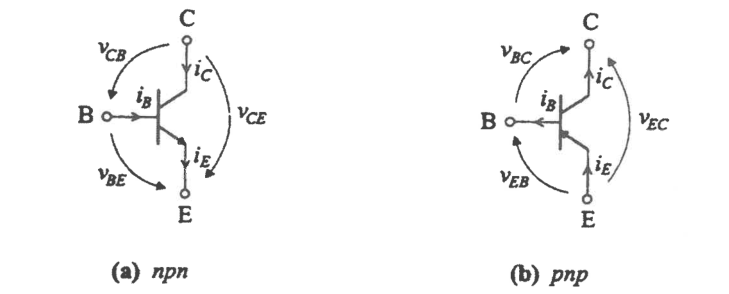
\includegraphics[width=0.7\linewidth]{img/3/BJT/BJT-symbol.png}
    \caption{``Símbolo dos transístores bipolares e sentidos de referência.''\cite{medeiros:CTBM}}
    \label{fig:BJT-symbol}
\end{figure}

\begin{quote}
    ``O funcionamento dos dois tipos de transístores é muito semelhante: quando se passa de um para o outro, todos os resultados se mantêm se se trocarem os sentidos das correntes e tensões.''\cite{medeiros:CTBM} 
\end{quote}

\noindent Na subsequente análise é \underline{considerado o transístor npn} dado que é o mais frequentemente utilizado.

\vspace{0.5em}
\noindent Das leis de Kirchhoff resulta que
$$
    \text{KCL}\; \boxed{ i_E = i_C + i_B } \mkern38mu \text{KVL}\; \boxed{ v_{CB} = v_{CE} - v_{BE} }
$$
$\implies$ para caracterizar o estado do transístor, basta indicar duas correntes e duas tensões.

%//==============================--@--==============================//%
\paragraph[3.1.1.1 Modo Ativo (ZAD)]{$\pmb{\star}$ Modo Ativo (ZAD)}\mbox{}

\begin{figure}[H]
    \centering
    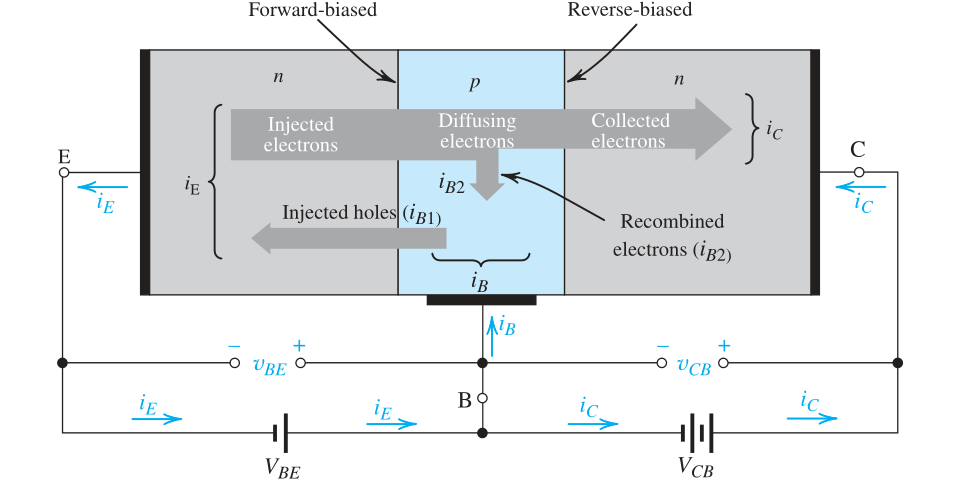
\includegraphics[width=0.75\linewidth]{img/3/BJT/active-mode.png}
    \caption{``Current flow in an npn transistor biased to operate in the active mode. (Reverse current
components due to drift of thermally generated minority carriers are not shown.)''\cite{sedra-smith:microelectronic-circuits}}
    \label{fig:active-mode}
\end{figure}

\noindent De modo a ilustrar o modo de operação do transístor no modo ativo, apresentam-se na \hyperref[fig:active-mode]{Fig. 21} duas fontes de tensão externas, $V_\textit{BE}$ e $V_\textit{CB}$, que verificam $v_\textit{CB} \ge v_\textit{BE}$.

\begin{itemize}[leftmargin=*]
    \item A tensão $V_\textit{BE}$ coloca a base de tipo p a um potencial superior ao emissor de tipo n, estabelecendo uma polarização direta na junção emissor-base (\textit{forward bias}). 
    
    \item A tensão coletor-base $V_\textit{CB}$, força o coletor de tipo n a um maior potencial relativamente à base, o que resulta numa polarização inversa para a junção coletor-base (\textit{reverse bias}).
\end{itemize}

\begin{itemize}[leftmargin=*]
    \item[] \textbf{Fluxo de corrente}:
    \begin{itemize}[leftmargin=*,label=$\pmb{-}$]
        \item A polarização direta da EBJ provoca o fluxo de corrente, composto por dois componentes: eletrões injetados do emissor para a base, e lacunas injetadas (de- sejavelmente, em menor quantidade) da base para o emissor.
        \item A magnitude da corrente do emissor, $i_E$, é dominada pelo componente maioritário (eletrões no caso do transístor npn).
        \begin{quote}
            ``The direction of $i_E$ is "out of" the emitter lead, which, following the usual conventions, is in the direction of the positive-charge flow (hole current) and opposite to the direction of the negative-charge flow (electron current), with the emitter current $i_E$ being equal to the sum of these two components. However, since the electron component is much larger than the hole component, the emitter current will be dominated by the electron component.''\cite{sedra-smith:microelectronic-circuits}
        \end{quote}
        \item As correntes do emissor e da base são proporcionais a $e^{v_\textit{BE}/V_T}$, onde $v_\textit{BE}$ é a tensão direta da junção base-emissor e $V_T \simeq 25$ mV é a tensão térmica (junção pn).
    \end{itemize}
    
    \item[] \textbf{Corrente do coletor}:
    \begin{itemize}[leftmargin=*,label=$\pmb{-}$]
        \item A maioria dos eletrões injetados do emissor para a base chega ao coletor, criando a corrente do coletor ($i_C$):
        $$
            i_C = I_S \left(e^{\frac{v_\textit{BE}}{V_T}} - 1\right) \simeq I_S\, e^{\frac{v_\textit{BE}}{V_T}},\quad \text{onde $I_S$ é a corrente de saturação}
        $$
    \end{itemize}
    
    \item[] \textbf{Corrente da base}:
    \begin{itemize}[leftmargin=*,label=$\pmb{-}$]
        \item A corrente da base ($i_B$) é composta por duas componentes: lacunas injetadas da base para o emissor e lacunas necessárias para o processo de \textbf{recombinação}\footnotemark[4] na base (também proporcionais a $e^{v_\textit{BE}/V_T}$). A corrente na base pode ser expressa como:
        $$
            i_B = \frac{i_C}{\beta},\quad \text{onde $\beta$ é o \textbf{ganho de corrente de emissor comum}}
        $$
    \end{itemize}
    
    \item[] \textbf{Corrente do emissor}:
    \begin{itemize}[leftmargin=*,label=$\pmb{-}$]
        \item A corrente do emissor ($i_E$) é a soma da corrente do coletor e da corrente da base.
        $$ i_E = i_C + i_B = \frac{\beta + 1}{\beta}\, i_C $$
        Alternativamente, é possível exprimir a fórmula na seguinte forma:
        $$ i_C = \alpha\, i_E $$
        em que a contante $\alpha$ se relaciona com $\beta$ por
        $$ \alpha = \frac{\beta}{\beta + 1} \iff \beta = \frac{\alpha}{1-\alpha}$$ 
        Como veremos mais adiante, $\alpha$ é também denominado por \textbf{ganho de corrente de base comum}.
    \end{itemize}
\end{itemize}

\footnotetext[4]{%
    Os eletrões injetados do emissor para a base são portadores minoritários na região da base tipo p. Durante a jornada até ao coletor, alguns eletrões combinam-se com lacunas (portadores de carga maioritários) na base. No entanto, como a base é geralmente muito fina e pouco dopada, a proporção de eletrões perdidos neste processo de recombinação é bastante pequena. A maioria dos eletrões difundidos alcança a fronteira da região de depleção coletor-base e, devido à tensão de polarização inversa ($v_\textit{CB}$) aplicada entre o coletor e a base, são varridos através da região de depleção, chegando finalmente ao coletor e constituindo a corrente do coletor $i_C$.
}

%//==============================--@--==============================//%
\paragraph[3.1.1.2 Modo de Saturação (\textit{Saturation})]{$\pmb{\star}$ Modo de Saturação (\textit{Saturation}\footnotemark[5])}\mbox{}

\vspace{-0.40em}
\begin{center}
    \begin{minipage}{0.65\linewidth}
        $v_{BE} = v_{CE} \simeq 0.7$V, de forma a que $i_C > 0$ e $i_B > 0$, mas $i_C < \beta i_B$. O transístor está plenamente saturado quando $v_{CE} = V_{CE\textit{sat}} = 0.2$V. 
        
        O circuito comporta-se como um \underline{interruptor fechado}.
    \end{minipage}%
    \qquad
    \raisebox{-0.5em}{%
    \begin{minipage}{0.25\linewidth}
        \begin{center}
            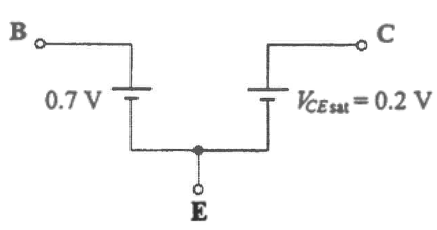
\includegraphics[width=1\linewidth]{img/3/BJT/saturation.png}
            \label{img:saturation-BJT}
        \end{center}
    \end{minipage}
    }
\end{center}

\footnotetext[5]{%
    ``Saturation means something completely different in a BJT and in a MOSFET. The saturation mode of operation of the BJT is analogous to the triode region of operation of the MOSFET. On the other hand, the saturation region of operation of the MOSFET corresponds to the active mode of BJT operation.''\cite{sedra-smith:microelectronic-circuits}
}

%//==============================--@--==============================//%
\vspace{-2.5em}
\paragraph[3.1.1.3 Modo de Corte (\textit{Cutoff})]{$\pmb{\star}$ Modo de Corte (\textit{Cutoff})}\mbox{}

\vspace{-1.25em}
\begin{center}
    \begin{minipage}{0.65\linewidth}
        $i_C = i_B = i_E = 0$ e o circuito equivalente é aberto.
        
        $v_{BE} < 0$ (tipicamente consideramos $v_{BE} < 0.5$V mediante a curva característica), e $v_{CE} > 0$. Como já explicitado $v_{BC} < 0$ já que possui polarização inversa.

        O circuito comporta-se como um \underline{interruptor aberto}.
    \end{minipage}%
    \qquad
    \begin{minipage}{0.25\linewidth}
        \begin{center}
            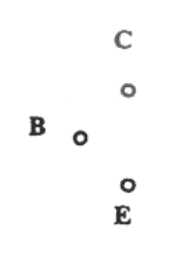
\includegraphics[width=0.6\textwidth]{img/3/BJT/cutoff.png}
            \label{img:cutoff-BJT}
        \end{center}
    \end{minipage}
\end{center}


%//==============================--@--==============================//%
\vspace{-2.0em}
\paragraph[3.1.1.4 TL;DR: Análise]{$\pmb{\star}$ TL;DR: Análise}\mbox{}\\[4pt]
Normalmente, é imediato verificar se o transístor se encontra em \underline{corte} ($v_\textit{BE} < 0.5$V) ou em \underline{condução} ($v_\textit{BE} \simeq 0.7$V). Torna-se mais difícil determinar se o circuito impõe o transístor, em condução, na ZAD ou na Zona de Saturação. Na prática \underline{assume-se uma das hipóteses} e verifica-se se os valores das tensões e correntes resultantes desta análise são congruentes com a suposição feita; caso não sejam, é porque se trata da outra zona de funcionamento (havendo que repetir a análise para obter os valores apropriados das tensões e correntes).

\begin{mdframed}
    \begin{itemize}[leftmargin=*]
        \item[] \textbf{(i) Corte:} \\
        $v_\textit{BE} \le 0.5$V; $i_B = 0$ e $i_C = 0 \implies i_E = 0$
        
        \item[] \textbf{(ii) Saturação:} \\
        $v_\textit{BE} \simeq 0.7$V; $v_\textit{CE} \le v_\textit{BE} \implies i_C < \beta i_B$
        $$
        \boxed{%
            v_\textit{CE} =
            \left\{\begin{aligned}
                v_\textit{BE} \simeq 0.7\text{V} &\rightarrow \text{limiar de saturação}\\
                V_\textit{CEsat} = 0.2\text{V} &\rightarrow \text{transístor profundamente saturado}
            \end{aligned}\right.
        }
        $$
        
        \item[] \textbf{(iii) Ativo (ZAD):} \\
        $v_\textit{BE} \simeq 0.7$V; $v_\textit{CE} > v_\textit{BE} \implies i_C = \beta i_B \;\land\; i_C = \alpha\, i_E$
        $$
        \boxed{%
            i_C = I_S(e^{\frac{v_\textit{BE}}{V_T}} - 1) \simeq I_S\, e^{\frac{v_\textit{BE}}{V_T}} \;\text{com } V_T = \frac{kT}{q} \simeq 25\,\text{mV ($@290$K)} 
        }
        $$
    \end{itemize}
\end{mdframed}

\noindent \underline{\textbf{Nota:}} O transístor é um elemento não-linear; cada zona de funcionamento pode ser aproximada por um esquema equivalente linear. A partir do momento em que se sabe a zona de funcionamento, basta aplicar as técnicas de análise de circuitos lineares para obter as correntes e tensões.

%//==============================--@--==============================//%
\newpage
\subsubsection[3.1.2 Curvas características i-v]{$\pmb{\rightarrow}$ Curvas características $\mathbf{i-v}$}
%//==============================--@--==============================//%
\vspace{-0.5em}
\paragraph[3.1.2.1 Característica iC-vBE e efeito da temperatura]{$\pmb{\star}$ Característica $\mathbf{i_C-v_{BE}}$ e efeito da temperatura}\mbox{}

\vspace{-0.5em}
\begin{figure}[H]
    \begin{subfigure}[b]{0.475\linewidth}
        \centering
        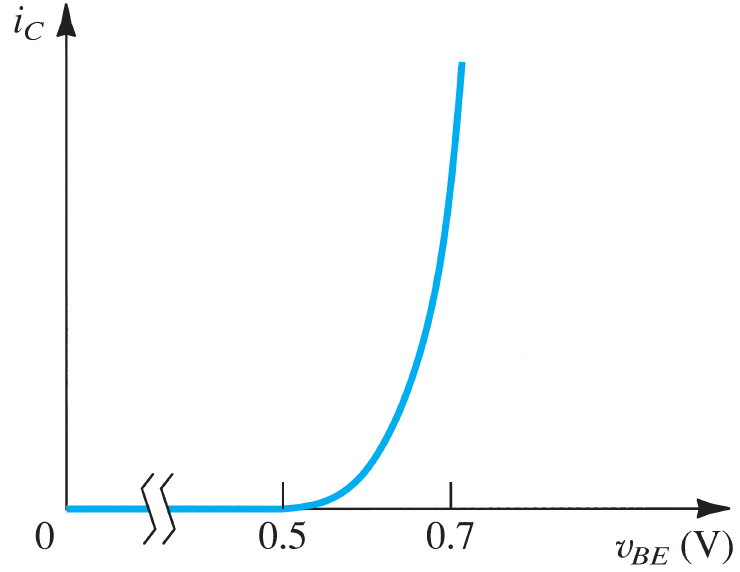
\includegraphics[width = 0.9\linewidth]{img/3/BJT/iC-vBE.png}
        \caption{Característica $i_C-v_\textit{BE}$ (npn). ``For $v_\textit{BE}$ smaller than about $0.5$V, the current is negligibly small (...)''\cite{sedra-smith:microelectronic-circuits}}
        \label{fig:i-vBE}
    \end{subfigure}\hfill
    \begin{subfigure}[b]{0.475\linewidth}
        \centering
        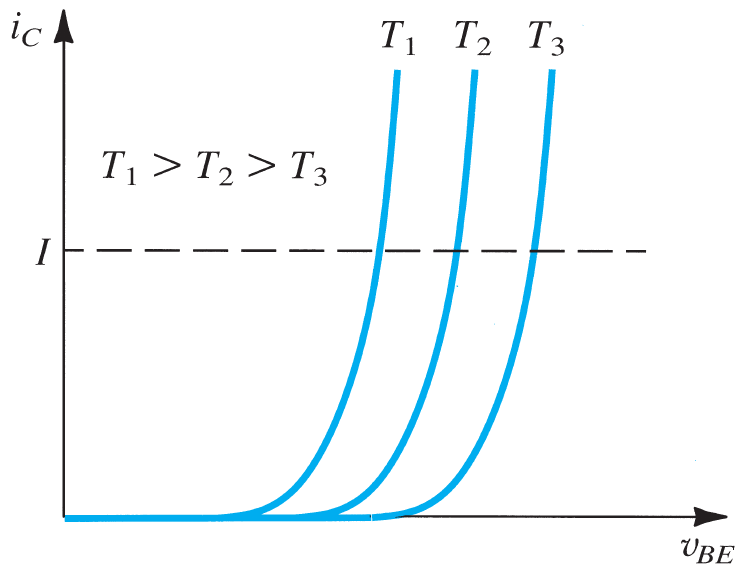
\includegraphics[width = 0.9\linewidth]{img/3/BJT/iC-vBE-T.png}
        \caption{``\textbf{Effect of temperature} (...) At a constant emitter current (broken
line), $v_\textit{BE}$ changes by $-2 \text{mV/\textdegree{C}}$.''\cite{sedra-smith:microelectronic-circuits}}
        \label{fig:i-vBE-T}
    \end{subfigure}%%
    \caption{Característica $i_C-v_\textit{BE}$}
    \label{fig:iC-vBE}
\end{figure}

\vspace{-1.75em}
\begin{quote}\small
    ``(...) over most of the normal current range $v_\textit{BE}$ lies in the range of $0.6$V to $0.8$V. In performing first-order DC calculations, we normally will assume that $V_\textit{BE} = 0.7$V, which is similar to the approach used in the analysis of diode circuits.''\cite{sedra-smith:microelectronic-circuits}
\end{quote}

%//==============================--@--==============================//%
\vspace{-1.5em}
\paragraph[3.1.2.2 Efeito de Early]{$\pmb{\star}$ Efeito de Early}\mbox{}

\vspace{-1em}
\begin{figure}[H]
    \centering
    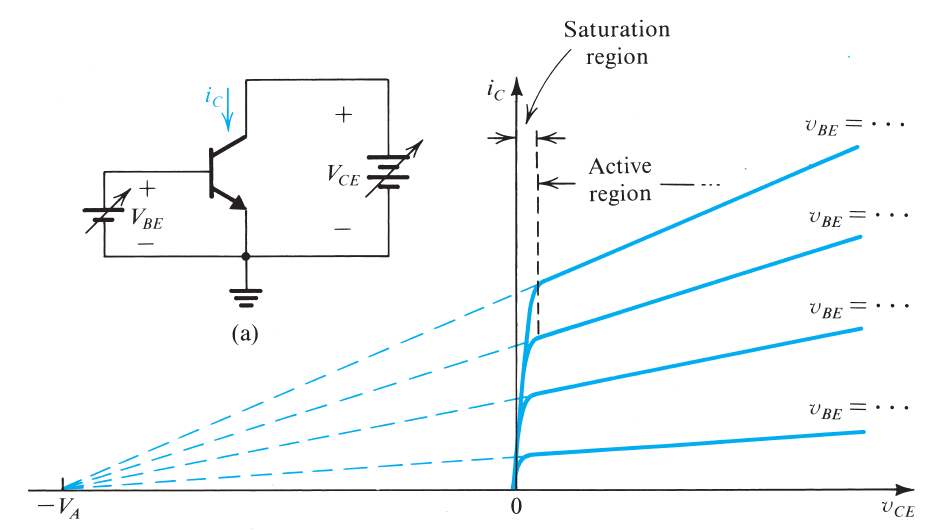
\includegraphics[width = 0.75\linewidth]{img/3/BJT/Early.png}
    \caption{Característica $i_C-v_{CE}$}
    \label{fig:Early}
\end{figure}

\vspace{-1.75em}
\begin{quote}\small
    ``At a given value of $v_{BE}$, increasing $v_{CE}$ increases the reverse-bias voltage on the collector–base junction, and thus increases the width of the depletion region of this junction. This in turn results in a decrease in the effective base width $W$. Recalling that $I_S$ is inversely proportional to $W$,\textbf{ we see that $I_S$ will increase and that $i_S$ increases proportionally}. This is the Early effect. For obvious reasons, it is also known as the base-width modulation effect.''\cite{sedra-smith:microelectronic-circuits}
\end{quote}

\noindent As curvas características atravessam o eixo das abcissas num ponto comum, $v_{CE} = -V_A$, onde $V_A$ é denominada de tensão de Early\footnotemark[6]. Esta dependência linear pode ser incutida na equação característica $i_C - v_{BE}$ da seguinte forma:
$$
    I_S\, \propto\, \frac{1}{W} \implies \boxed{i_C = I_S\, e^{v_{BE}/V_T} \left(1 + \frac{v_{CE}}{V_A}\right)}
$$

\footnotetext[6]{%
    ``The voltage $V_A$, a positive number, is a parameter for the particular BJT. As noted earlier, it is called the \textbf{Early voltage}, after J. M. Early, the engineering scientist who first studied this phenomenon''\cite{sedra-smith:microelectronic-circuits}
}

%//==============================--@--==============================//%
\newpage
\subsubsection[3.1.3 Esquema incremental]{$\pmb{\rightarrow}$ Esquema incremental}

Os circuitos analógicos destinam-se, na maior parte dos casos, a realizar operações \underline{lineares}. Nestes circuitos, \underline{pretende-se que os transístores se encontrem na ZAD}, podendo as suas tensões e correntes variar, mas sempre de modo a que o modo de funcionamento permaneça sobre um troço linear das curvas que caracterizam o funcionamento do transístor na ZAD.

Os sinais de interesse são as \underline{pequenas variações} das tensões e correntes, e não o total.

\begin{mdframed}
    \noindent Diz-se que o circuito está em \underline{repouso quando as componentes variáveis são nulas}. As componentes contínuas definem o \textbf{ponto de funcionamento em repouso} (PFR).
\end{mdframed}

\vspace{-0.25em}
\begin{figure}[H]
    \centering
    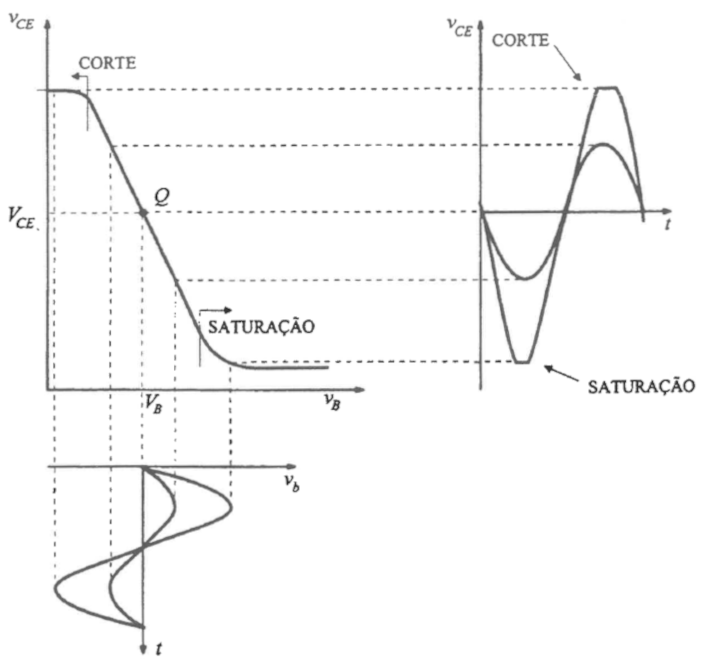
\includegraphics[width = 0.6\linewidth]{img/3/BJT/funcionamento-dinamico.png}
    \caption{Funcionamento dinâmico linear e não-linear \cite{medeiros:CTBM}}
    \label{fig:funcionamento-dinamico}
\end{figure}

\noindent Quando a tensão de saída não tem a forma da tensão de entrada, então há \underline{distorção}, resultante do funcionamento não-linear. A \underline{margem dinâmica} é dada pelas amplitude máximas incrementais para o qual ainda não ocorre distorção. Este valor é normalmente maximizado para o PFR localizado a meio do troço linear da característica (neste caso o corte e a saturação manifestam-se para as mesmas amplitudes da tensão de entrada).
\vspace{1em}\hrule\vspace{1em}
\noindent O uso de um \underline{esquema equivalente incremental} (interessa-nos o \textbf{esquema em $\pmb{\pi}$ híbrido}) pressupõe uma análise do funcionamento dinâmico linear do circuito, que ocorre quando as componentes variáveis têm amplitude limitada, de modo a que o ponto de funcionamento do transístor permaneça sobre um troço aproximadamente linear das suas características. Diz-se, neste caso, que o circuito tem \textbf{sinais fracos}.

\vspace{1 em}
\noindent Neste funcionamento o transístor é caracterizado por \textbf{parâmetros incrementais}, que caracterizam o seu modelo equivalente, $g_m$ e $r_\pi$:
$$
    \boxed{i_c = g_m\, v_{\pi}} \quad\land\quad \boxed{v_{\pi} = r_\pi\, i_b}
$$

\newpage
\begin{mdframed}
    \noindent Supondo que $i_C = I_C + i_c$ e $v_{BE} = V_{BE} + v_{be}$, e relembrando a característica $i_C-v_{BE}$ já discutida anteriormente, obtemos (desprezando o efeito de Early):

    \vspace{-0.25em}
    \begin{center}
        \begin{minipage}{0.3\linewidth}
            $$
                \boxed{i_C = I_se^{(V_{BE} + v_{be})/ V_T}}  \;\rightarrow\;
            $$
        \end{minipage}%
        \raisebox{-0.75em}{%
        \begin{minipage}{0.6\linewidth}
            A exponencial associada a $v_{be}$ é aproximada por $1 + v_{eb}/V_T$, já que $v_{be}$ se trata de um sinal fraco ($v_{eb} \ll V_T\:$ e $\:[e^x \simeq 1-x\;\text{\small (Maclaurin de 1\textordfeminine{}. ordem)}]$).
        \end{minipage}}
    \end{center}

    \vspace{-0.5em}
    \noindent Finalmente, admitimos que:
    $$
        i_C = I_C + i_c = I_se^{V_{BE}/ V_T}(1 + v_{eb}/V_T)\;
        \rightarrow\; \boxed{i_c = \dfrac{I_C}{V_T} v_{eb}}
    $$
\end{mdframed}

\renewcommand*{\thefootnote}{\fnsymbol{footnote}}
\footnotetext[4]{%
    \textbf{Nota:} As correntes e tensões no transístor têm uma componente contínua e uma componente variável. De acordo com a notação utilizada na literatura, o \textbf{valor total} será representado por uma letra minúscula com índice maiúsculo (e.g.: $v_B$), o \textbf{valor em repouso} ou \textbf{componente contínua} será representado por uma letra maiúscula com índice maiúsculo (e.g.: $V_B$) e o \textbf{valor incremental} por uma letra minúscula com índice minúsculo (e.g.: $v_b$).
}
\renewcommand*{\thefootnote}{\arabic{footnote}}

\noindent Donde resulta que a \textbf{transcondutância} é:
$$
    \boxed{g_m = \left.\frac{\partial i_C}{\partial v_\textit{BE}}\right|_{v_\textit{BE} = V_\textit{BE};\, v_\textit{CE} = V_\textit{CE}} \simeq I_C/V_T}
$$

\noindent O parâmetro $g_m$ depende apenas do \textbf{ponto de funcionamento em repouso} (PFR). Na caracterização da maior parte dos circuitos lineares, $g_m$, tem um papel determinante (e.g., o ganho de tensão do andar de emissor comum é proporcional a $g_m$). Interessa, por isso, que o valor em repouso seja bem definido e estável.

\begin{mdframed}
    \noindent Para determinar $r_\pi$ consideramos o transístor na zona ativa:
    $$
        i_c = \beta i_b
    $$
    \noindent Recordando a relação linear entre $i_c$ e $g_m$:
    $$
        v_{\pi} = r_\pi i_b = \frac{\beta}{g_m} i_b \implies \boxed{r_\pi = \frac{\beta}{g_m}}
    $$
    \noindent Note-se que $r_\pi$, depende do ponto de funcionamento em repouso (tal como $g_m$) e também da tecnologia (através de $\beta$).
\end{mdframed}

\noindent Na realidade, $i_C$ também depende de $v_\textit{CE}$, embora de modo não muito acentuado, como mencionado anteriormente. Isto constitui o \textbf{efeito de Early}. As características $i_C(v_\textit{CE})$ com $v_{BE}$ constante são aproximadamente retilíneas na zona ativa, mas não são horizontais; se fossem prolongadas para valores negativos de $v_\textit{CE}$ cortariam o eixo das abcissas em $-V_A$. Assim, a equação do transístor considerando o efeito de Early é:
$$
    \boxed{i_C = I_S\, e^{v_{BE}/V_T} \left(1 + \frac{v_{CE}}{V_A}\right)}
$$
O parâmetro $V_A$ (tensão de Early) está normalmente compreendido entre $50$ e $150$V. Quando se despreza o efeito de Early $V_A \to +\infty$.

{\setlength{\fboxrule}{2pt} 
\begin{minipage}{\linewidth}
    \raisebox{1.75em}{%
    \begin{minipage}[t]{0.475\linewidth}
        \begin{figure}[H]
            \centering
            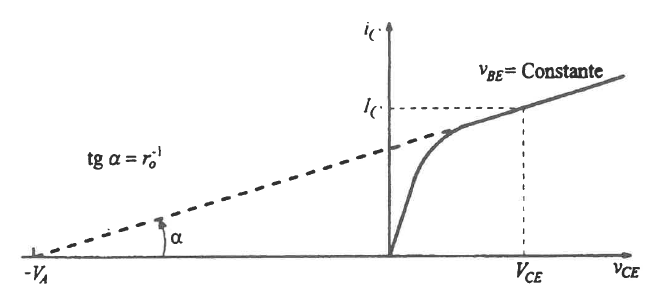
\includegraphics[width=\linewidth]{img/3/BJT/efeito-Early.png}
            \captionsetup{skip=-2pt}
            \caption{Efeito de Early \cite{medeiros:CTBM}}
            \label{fig:efeito-early-declive}
        \end{figure}
    \end{minipage}}\hspace*{1pt}
    \noindent\fbox{%
    \begin{minipage}[t]{0.46\linewidth} \small
        A inclinação da característica é:
        $$
            r_o^{-1} = \left.\frac{\partial i_C}{\partial v_\textit{CE}}\right|_{v_\textit{BE} = V_\textit{BE};\, v_\textit{CE} = V_\textit{CE}} = \frac{I_C}{V_A + V_\textit{CE}}
        $$
        e como $V_A \gg V_\textit{CE}$ tem-se, aproximadamente:
        $$
            r_o \simeq \frac{V_A}{I_C}\; \text{\small (novo parâmetro incremental)}
        $$
    \end{minipage}}
\end{minipage}
}

\vspace{0.25em}
\noindent A expressão da transcondutância \underline{não é alterada quando se considera o efeito de Early}. Quando se considera este efeito, há que introduzir no esquema incremental do transístor a resistência $r_o$ entre o coletor e o emissor de modo a traduzir a influência de $v_\textit{ce}$ sobre $i_c$.

Usualmente o efeito de Early afeta pouco o funcionamento em repouso, mas pode afetar muito o funcionamento dinâmico (principalmente no caso dos circuitos integrados).

\begin{figure}[H]
    \begin{subfigure}[b]{0.5\linewidth}
        \centering
        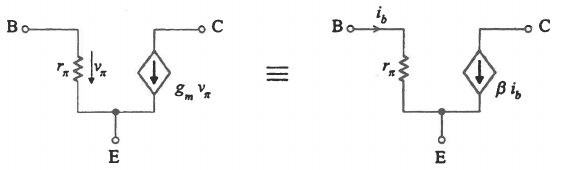
\includegraphics[width = \linewidth]{img/3/BJT/esquema-incremental.png}
        \caption{Esquema incremental em $\pi$ \cite{medeiros:CTBM}}
        \label{fig:esquema-incremental}
    \end{subfigure}%%
    \begin{subfigure}[b]{0.5\linewidth}
        \centering
        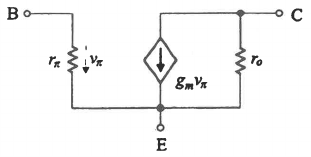
\includegraphics[width = 0.55\linewidth]{img/3/BJT/esquema-incremental-Early.png}
        \caption{Esquema incremental considerando o efeito de Early \cite{medeiros:CTBM}}
        \label{fig:esquema-incremental-Early}
    \end{subfigure}
    \caption{Esquemas incrementais em $\pi$}
    \label{fig:esquemas-incrementais}
\end{figure}

\vspace{-0.5em}
\noindent Dado que $r_o \simeq V_A/I_C$ e $g_m = I_C/V_T$,  vem que: 
$$
    \frac{r_o}{g_m^{-1}} = \frac{V_A}{V_T}
$$
\noindent Como $r_\pi = \beta\, g_m^{-1}$, para os valores usuais dos parâmetros incrementais, podemos concluir:
$$
    \boxed{r_o \gg r_\pi \gg g_m^{-1}}
$$

\begin{mdframed} \small
    \noindent O \textbf{esquema incremental do transístor} é muito útil para analisar circuitos em regime dinâmico linear (com \textbf{sinais fracos}). Esta análise efectua-se, com comodidade, substituindo o circuito pelo seu esquema equivalente do ponto de vista incremental, o qual se obtém do seguinte modo:
    \begin{enumerate}[leftmargin=*] \small
        \item Os transístores são substituídos pelo seu esquema incremental. Se, para além dos transístores, existirem outros dispositivos não-lineares (por exemplo, díodos), estes são também substituídos pelos seus esquemas incrementais.
    
        \item As fontes de tensão contínua são substituídas por curto-circuitos, pois a componente incremental de uma tensão constante é nula; as fontes de corrente contínua são substituídas por circuitos abertos, com análoga justificação.
        
        \item Os elementos lineares (resistências, condensadores, etc) mantêm-se, uma vez que eles coincidem com o seu esquema incremental (as equações que os descrevem em termos dos valores totais são lineares e, por isso, são aplicáveis aos valores incrementais).
    \end{enumerate}
\end{mdframed}

\renewcommand*{\thefootnote}{\fnsymbol{footnote}}
\footnotetext[4]{%
    ``E importante notar que \textbf{os esquemas incrementais dos transístores \textit{pnp} e \textit{npn} são idênticos}. Pode considerar-se que os sentidos das correntes e tensões incrementais são os mesmos nos dois tipos de transístores (embora tal não seja verdade para os valores totais).''\cite{medeiros:CTBM}
}
\renewcommand*{\thefootnote}{\arabic{footnote}}

%//==============================--@--==============================//%
\subsubsection[3.1.4 Polarização Estabilizada]{$\pmb{\rightarrow}$ Polarização Estabilizada}



%//==============================--@--==============================//%
        \clearpage
%//==============================--@--==============================//%
\subsection[3.2 Transístor MOS (MOSFET)]{\hspace*{0.075 em}\raisebox{0.2 em}{$\pmb{\drsh}$} Transístor MOS (MOSFET)}
\label{subsec:transistor-MOS}

O \textbf{transístor de efeito de campo} (\textit{Field Effect Transistor}, acrónimo FET) tem esta designação porque o estado de corte ou de condução é determinado pelo campo elétrico no seu interior. A corrente deve-se a um só tipo de portadores de carga (eletrões ou lacunas), ao contrário do que se sucede com os BJT.

Existem vários tipos de transístores de efeito de campo, dos quais o mais utilizado é, de longe, o transístor \textbf{MOS} (MOSFET); a designação MOS provém das iniciais de Metal-Oxide-Semicondutor. 

\vspace{0.5em}
\noindent Algumas considerações pertinentes:
\begin{itemize}[leftmargin=*, nolistsep, itemsep=1pt, label=\rule{0.9ex}{0.9ex}]
    \item Os transístores MOS ocupam menor área, apresentam uma resistência de entrada praticamente infinita, funcionam melhor como interruptores e permitem realizar circuitos digitais com menor consumo (afinidade à realização de circuitos digitais).
    
    \item Os transístores bipolares permitem obter maior ganho, maior largura de banda e precisão mais elevada (especialmente vocacionados para a realização de circuitos analógicos). 

    \item No entanto, \underline{esta separação} dos domínios de aplicação dos dois tipos de transístores está atualmente \underline{ultrapassada}.

    \item Os transístores MOS, inicialmente usados em circuitos lógicos e memórias, são também usados correntemente na realização de circuitos analógicos (descobriram-se formas engenhosas de implementar funções digitais e analógicas quase exclusivamente com MOSFETs $[$i.e., com muito poucas ou nenhumas resistências$]$).

    \item Os transitares bipolares continuam a ser usados na realização de circuitos analógicos e são também usados na realização de circuitos digitais, principalmente se estes tiverem de ser muito rápidos. 

    \item Existem atualmente tecnologias \textbf{BiCMOS}, que combinam, no mesmo circuito integrado, transístores bipolares e CMOS.
\end{itemize}

\begin{figure}[H]
    \begin{subfigure}[b]{0.5\linewidth}
        \centering
        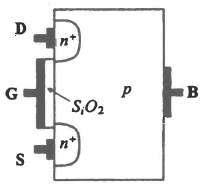
\includegraphics[width = 0.6\linewidth]{img/3/MOSFET/NMOS-enhancement.png}
        \caption{NMOS de reforço}
        \label{fig:NMOS-enhancement}
    \end{subfigure}
    \begin{subfigure}[b]{0.5\linewidth}
        \centering
        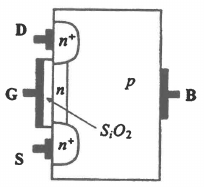
\includegraphics[width = 0.6\linewidth]{img/3/MOSFET/NMOS-depletion.png}
        \caption{NMOS de depleção}
        \label{fig:NMOS-depletion}
    \end{subfigure}%%
    \caption{Estrutura física dos transístores NMOS de reforço e de depleção}
    \label{fig:NMOS}
\end{figure}

\noindent A estrutura básica de um MOSFET inclui um \textbf{substrato} ou corpo (\textit{body}), sobre o qual estão o \textbf{dreno} (\textit{drain}) e a \textbf{fonte} (\textit{source}), áreas altamente concentradas de um tipo de semicondutor. Entre o dreno e a fonte, há uma camada isolante de óxido de silício (SiO$_{2}$), e acima desta, uma camada condutora que constitui a \textbf{porta} (\textit{gate}). 

A corrente flui do dreno para a fonte quando a tensão entre a porta e a fonte, $v_{GS}$, é superior à \textbf{tensão de limiar} (\textit{threshold}), $V_{t}$, formando assim um \textbf{canal}\footnotemark[7] condutor.

\footnotetext[7]{%
    Nos transístores MOS de \textbf{reforço} (\textit{enhancement}) o controlo da corrente obtém-se ao trazer mais ou menos portadores de carga para o canal. Para os MOS de \textbf{depleção}  (\textit{depletion}), o canal é criado durante a fabricação do circuito; o controlo faz-se afastando mais ou menos portadores de carga.
}

\newpage
\noindent \textbf{Notas sobre o funcionamento} dos MOSFET:
\begin{itemize}[leftmargin=*, nolistsep, itemsep=1pt, label=\rule{0.9ex}{0.9ex}]
    \item Contrariamente ao que se verifica nos transístores bipolares, os MOSFET de baixa potência têm uma \underline{estrutura simétrica} (os transístores MOS de potência são assi- métricos). Assim, o dreno e a fonte são determinados pela polaridade da tensão existente entre eles. 

    \item Devido à presença da camada isolante sob a porta, o terminal desta não é percorrido por corrente, i.e., $i_G = 0$. O substrato também não apresenta corrente, porque as suas junções com o dreno e a fonte estão polarizadas em sentido inverso. 
    
    (Normalmente o substrato está ligado à fonte, ou ao terminal negativo da alimentação)

    \item Como $i_G = 0$ e $i_B = 0$, \underline{as correntes na fonte e no dreno são iguais}, $i_D = i_S$.
\end{itemize}

\begin{mdframed}
    \noindent Existem múltiplos \textbf{símbolos} utilizados para representar os transístores MOS. Na \hyperref[fig:MOS-simbolos]{figura seguinte} apresenta-se a simbologia mais antiga (em cima), e a representação frequentemente utilizada atualmente (em baixo).

    \begin{figure}[H]
        \centering
        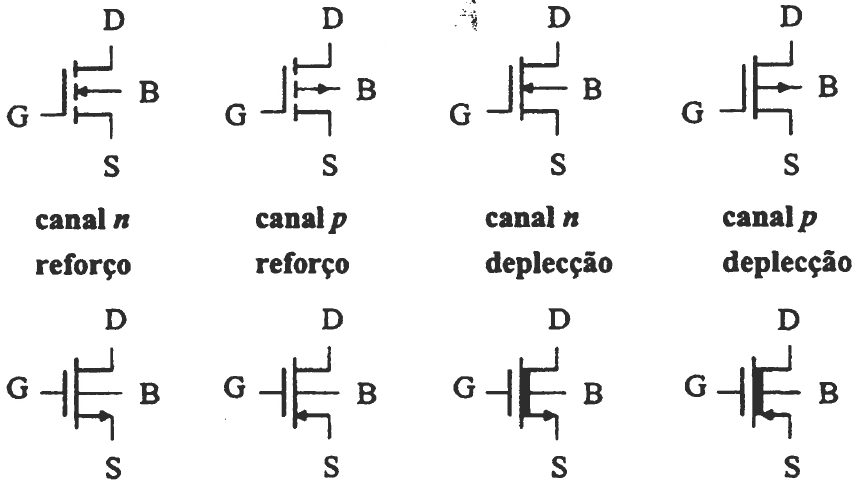
\includegraphics[width=0.7\linewidth]{img/3/MOSFET/MOS-simbolos.png}
        \caption{Símbolos dos transístores MOS \cite{medeiros:CTBM}}
        \label{fig:MOS-simbolos}
    \end{figure}

    \noindent Quando não é necessário indicar o terminal do substrato, recorre-se à representação \textbf{simplificada}, que o omite (dado que não é percorrido por corrente e é ligado à fonte ou a uma tensão fixa):

    \begin{figure}[H]
        \centering
        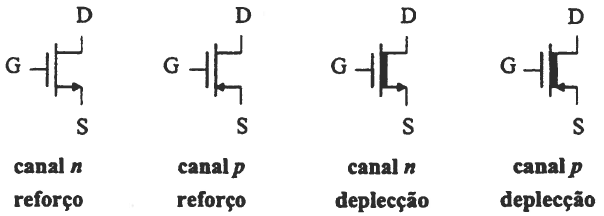
\includegraphics[width=0.65\linewidth]{img/3/MOSFET/MOS-simbolos-simplificado.png}
        \caption{Representação simplificada dos transístores MOS \cite{medeiros:CTBM}}
        \label{fig:MOS-simbolos-simplificado}
    \end{figure}
\end{mdframed}

%//==============================--@--==============================//%
\newpage
\subsubsection[3.2.1 Modos de funcionamento e características i-v]{$\pmb{\rightarrow}$ Modos de funcionamento e características $\mathbf{i-v}$}

\vspace{-0.75em}
\begin{figure}[H]
    \centering
    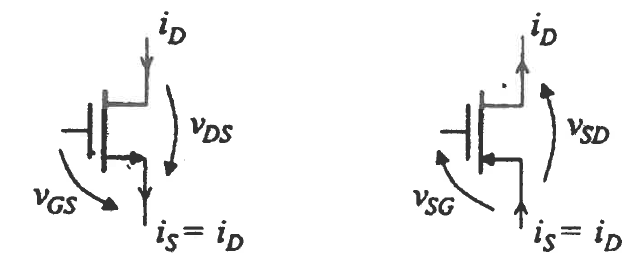
\includegraphics[width=0.55\linewidth]{img/3/MOSFET/MOS-sentidos.png}
    \caption{Sentidos de referência \cite{medeiros:CTBM}. Os sentidos de referência adotados foram escolhidos de forma a que as correntes sejam sempre positivas. Não há corrente aos terminais da porta e do substrato, $i_G = i_B = 0$.}
    \label{fig:MOS-sentidos}
\end{figure}

\vspace{-0.75em}
\noindent Os sentidos de referência para os transístores de depleção são iguais aos apresentados para os transístores de reforço. No entanto, a tensão de limiar $V_t$ passa a ser negativa, podendo os transístores conduzir com $v_{GS} < 0$ ou $v_{SG} < 0$, desde que estas tensões sejam superiores a $V_t$.

\phantomsection\addcontentsline{toc}{paragraph}{Zonas de funcionamento}
\begin{theo}[\underline{Zonas de funcionamento}]{def:MOS-zonas}\label{def:MOS-zonas}
    \begin{itemize}[leftmargin=*]
        \item[] \textbf{(i) Corte:} \hfill $\boxed{ v_{GS} < V_t \rightarrow i_D = i_S = 0}$ \\[1pt]
        Não existem\footnotemark[8] portadores entre D e S
        
        \item[] \textbf{(ii) Condução:} \hfill $\boxed{ v_{GS} > V_t \rightarrow i_D = i_S \neq 0}$ \\[1pt]
        Quando os transístores MOS conduzem podem situar-se em duas regiões de funcionamento: \\
        Região de \textbf{tríodo} (ou óhmica) e a região de \textbf{saturação} (ou de estrangulamento).
        
        \begin{itemize}[label=\rule{0.9ex}{0.9ex}]
            \item O transístor NMOS está na região de \textbf{tríodo} \hfill $\boxed{ v_{DS} < v_{GS} - V_t }$

            Neste caso a corrente é dada por
            $$
                \boxed{ i_D = k\left[ 2(v_{GS} - V_t)v_{DS} - v_{DS}^2 \right] }
            $$
            em que $k$ é um parâmetro dependente do material e da geometria do transístor.

            Note-se que para tensões $v_{DS} \ll v_{GS} - V_t$, o transístor comporta-se como uma resistência $R_{DS}$ comandada pela tensão $v_{GS}$:
            $$
                i_D \approx 2k(v_{GS} - V_t)v_{DS} \implies R^{-1}_{DS} = 2k(v_{GS} - V_t)
            $$

            \item O transístor NMOS está na região de \textbf{saturação} \hfill $\boxed{ v_{DS} \ge v_{GS} - V_t }$

            A corrente passa a ser aproximadamente independente de $v_{DS}$:
            $$
                \boxed{ i_D = k\left( v_{GS} - V_t \right)^2 }
            $$
        \end{itemize}
        
    \end{itemize}
\end{theo}
      
\noindent O parâmetro $k$ que figura nas equações anteriores exprime-se em AV$^{-2}$
$$
    \boxed{ k = \frac{1}{2}\, \mu C_{ox} \frac{W}{L} } \;\: \text{em que }\, C_{ox} = \frac{\varepsilon_{ox}}{t_{ox}}\; \text{\footnotesize (capacidade formada entre a porta e o substrato)}
$$

\footnotetext[8]{%
    ``This is not entirely true, for it has been found that for values of $v_{GS}$ smaller than but close to $V_t$, a small drain current flows. In this \textbf{subthreshold} region of operation, the drain current is exponentially related to $v_{GS}$, much like the $i_C-v_{BE}$ relationship of a BJT''\cite{sedra-smith:microelectronic-circuits}
}

\renewcommand*{\thefootnote}{\fnsymbol{footnote}}
\footnotetext[4]{%
    $W$ é a largura (\textit{width}) do transístor, e $L$ o comprimento (\textit{length}). $W/L$ refere-se como \textit{aspect-ratio}.
}
\renewcommand*{\thefootnote}{\arabic{footnote}}
%//==============================--@--==============================//%
\paragraph[3.2.1.1 Características i-v]{$\pmb{\star}$ Características $\mathbf{i-v}$}\mbox{}\\[4pt]
A representação gráfica das características $i_D(v_{DS})$ para diferentes valores de $v_{GS}$ é acompanhada pela região de fronteira entre as regiões tríodo e de saturação

\vspace{-0.75em}
$$
    v_{DS} = v_{GS} - V_t\;\; \text{donde resulta}\;\; i_D = k\, v^2_{DS}
$$

\vspace{-0.75em}
\begin{figure}[H]
    \begin{subfigure}[b]{0.5\linewidth}
        \centering
        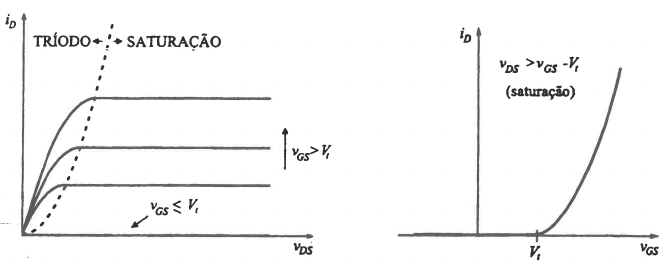
\includegraphics[width = 0.95\linewidth]{img/3/MOSFET/i-v-enhancement.png}
        \caption{Características do NMOS de reforço}
        \label{fig:NMOS-i-v-enhancement}
    \end{subfigure}
    \begin{subfigure}[b]{0.5\linewidth}
        \centering
        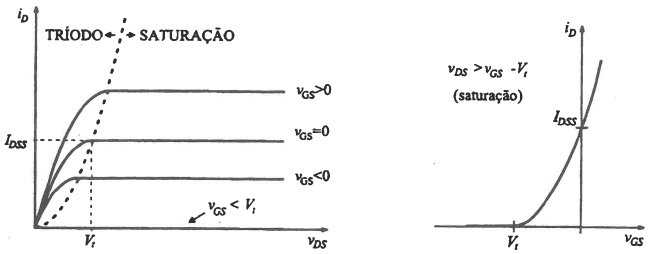
\includegraphics[width = 0.95\linewidth]{img/3/MOSFET/i-v-depletion.png}
        \caption{Características do NMOS de depleção}
        \label{fig:NMOS-i-v-depletion}
    \end{subfigure}%%
    \caption{Características $i-v$ para o transístor NMOS}
    \label{fig:NMOS-i-v}
\end{figure}

\noindent Os transístores de depleção têm as mesmas equações que os de reforço, mas como mencionado anteriormente, a tensão de limiar $V_t$ é negativa. Desta forma, costuma representar-se $I_{DSS} = kV^2_t$ (\textit{drain current for zero bias}), o valor de $i_D$ quando $v_{GS} = 0$. Para valores de $v_{GS} < 0$, encontra-se no modo de depleção, e para $v_{GS} > 0$ no de reforço. 

\begin{figure}[H]
    \centering
    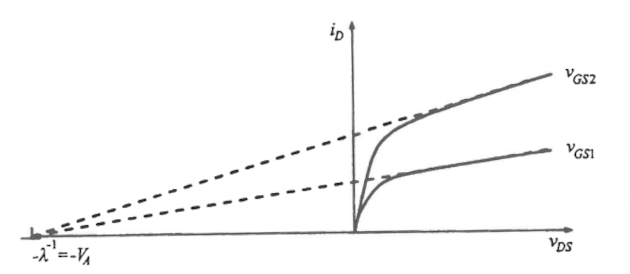
\includegraphics[width = 0.6\linewidth]{img/3/MOSFET/MOS-early-effect.png}
    \caption{Efeito de $v_{DS}$ sobre $i_{D}$ na saturação \cite{medeiros:CTBM}}
    \label{fig:MOS-early-effect}
\end{figure}

\noindent Na realidade, a tensão $v_{DS}$ tem alguma influência em $i_D$. Isto resulta do fenómeno designado por \underline{modulação do comprimento do canal}, cujas consequências são semelhantes ao efeito de Early (modulação da espessura da base) nos BJT.

Caso se considere este efeito, a característica \underline{na região de saturação} passa a ser
$$
    \boxed{ i_D = k\left( v_{GS} - V_t \right)^2 (1 + \lambda v_{DS}) }
$$
em que o parâmetro $\lambda^{-1} = V_A$ é equivalente à tensão de Early nos transístores bipolares.

%//==============================--@--==============================//%
\paragraph[3.2.1.2 Efeito da Temperatura]{$\pmb{\star}$ Efeito da Temperatura}\mbox{}\\[4pt]
Os parâmetros $V_t$ e $k$ que caracterizam o transístor MOS são sensíveis à temperatura: a tensão de limiar $V_t$, diminui cerca de $2$mV/\textdegree{C}; o parâmetro $k$ também diminui com a temperatura, e o seu efeito sobre $i_D$ opõe-se e predomina sobre o da variação de $V_t$. Assim, com $i_D$ constante, $v_{GS}$ aumenta com a temperatura. Note-se que este efeito é ao contrário do que acontece no transístor bipolar, em que, com $i_C$ constante, $v_{BE}$ diminui quando aumenta a temperatura.

%//==============================--@--==============================//%
\newpage
\paragraph[3.2.1.3 Efeito de Corpo]{$\pmb{\star}$ Efeito de Corpo (\textit{Body Effect})}\mbox{}\\[4pt]
O \textbf{efeito de corpo}, ou \textit{body effect}, relaciona a alteração da tensão de limiar do dispositivo, $V_t$, com a tensão aplicada ao substrato (ou corpo). Esta alteração é especialmente notável quando o substrato não está ligado ao \textit{ground} ou está ligado a um potencial diferente do terminal da fonte.

\begin{mdframed}
    \noindent A tensão de limiar modificada devido ao \textbf{efeito de corpo} é representada por:
    
    $$
        \boxed{ V_t = V_{t0} + \gamma \left[ \sqrt{{2\phi_f + v_{SB}}} - \sqrt{{2\phi_f}} \right] }
    $$
    
    \noindent em que:
    \begin{itemize}[noitemsep, nolistsep]
        \item $V_{t0}$ é a tensão de limiar \underline{sem o efeito de corpo}.
        \item $\gamma$ é o coeficiente do efeito de corpo, também conhecido como parâmetro de modulação do substrato (depende da técnologia).
        \item $\phi_f$ é o potencial de Fermi.
    \end{itemize}
    
    \vspace{0.5em}
    \noindent A equação acima indica que a tensão de limiar aumenta com o aumento de $v_{SB}$. Este efeito é normalmente indesejável em aplicações analógicas, porque introduz não-linearidades. Em aplicações digitais, onde os transístores operam em modo de corte ou saturação, o efeito é menos relevante.
\end{mdframed}

%//==============================--@--==============================//%
\subsubsection[3.2.2 Modelo incremental]{$\pmb{\rightarrow}$ Modelo incremental}

À semelhança da discussão realizada para os BJT, se o transístor permanecer na região de saturação temos
$$
    \begin{aligned}
        i_D = (I_D + i_d) &= k(V_{GS} + v_{gs} - V_t)^2\\
        &= k(V_{GS} - V_t)^2 + 2k(V_{GS} - V_t) v_{gs} + k v^2_{gs}
    \end{aligned}
$$
\noindent como $I_D = k(V_{GS} - V_t)^2$, fica
$$
    i_d = 2k (V_{GS} - V_t)v_{gs} + k v^2_{gs}
$$
O funcionamento é linear do ponto de vista incremental se $v_{gs} \ll V_{GS} - V_t$, obtendo-se
$$
    i_d = g_m v_{gs}
$$
em que a \textbf{transcondutância} $g_m$, é dada por
$$
    g_m = 2k(V_{GS} - V_t) \iff g_m = 2\sqrt{k I_D}
$$
Se considerarmos o efeito de $v_{DS}$ sobre $i_D$, a transcondutância define-se como
$$
    g_m = \left.\frac{\partial i_D}{\partial v_{GS}}\right|_{v_{GS} = V_{GS};\; v_{DS} = V_{DS}} = 2k(V_{GS} - V_t)(1 + \lambda V_{DS}) = \frac{2 I_D}{V_{GS} - V_t}
$$
\noindent \textbf{Nota:} se $\lambda V_{DS} \ll 1$, o resultado coincide com o anterior, como seria esperado.

\vspace{0.5em}
\noindent Para se ter em conta o efeito de $v_{ds}$ sobre $i_d$ é necessário introduzir o parâmetro incremental
$$
    r^{-1}_o = \left.\frac{\partial i_D}{\partial v_{DS}}\right|_{v_{GS} = V_{GS};\; v_{DS} = V_{DS}} \implies r_o = \frac{1 + \lambda V_{DS}}{\lambda I_D} \;\overset{\scriptstyle \lambda V_{DS} \ll 1}{\simeq}\; \frac{1}{\lambda I_D} = \frac{V_A}{I_D}
$$

\newpage
\noindent Se o \textbf{efeito de corpo} não for desprezável, i.e., a tensão entre a fonte e o substrato não for constante, $v_{bs} \neq 0$, representa-se no esquema incremental um gerador de corrente comandado extra, com parâmetro incremental $g_{mb}$ que se situa entre $0.1 g_m$ e $0.3 g_m$:
$$
    g_{mb} = \left.\frac{\partial i_D}{\partial v_{BS}}\right|_{v_{GS} = V_{GS};\; v_{DS} = V_{DS};\; v_{BS} = V_{BS}}
$$

\begin{figure}[H]
    \begin{subfigure}[b]{0.5\linewidth}
        \centering
        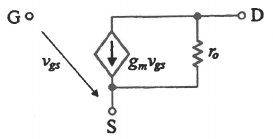
\includegraphics[width = 0.85\linewidth]{img/3/MOSFET/MOS-esquema-ro.png}
        \caption{Com o efeito de $v_{ds}$ sobre $i_d$ ($\lambda \neq 0$)}
        \label{fig:MOS-esquema-ro}
    \end{subfigure}
    \begin{subfigure}[b]{0.5\linewidth}
        \centering
        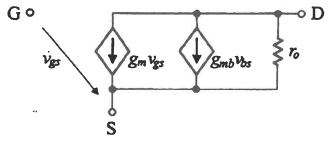
\includegraphics[width = \linewidth]{img/3/MOSFET/MOS-esquema-body.png}
        \caption{Quando há efeito de corpo}
        \label{fig:MOS-esquema-body-effect}
    \end{subfigure}%%
    \caption{Esquemas incrementais para os transístores MOS \cite{medeiros:CTBM}}
    \label{fig:MOS-esquema-incremental}
\end{figure}

\begin{mdframed}
    \begin{quote} \small
        ``É oportuno fazer a comparação das transcondutâncias dos transístores bipolar e MOS. $[$Sem o efeito de corpo temos:$]$
        $$
            \frac{(g_m)_{BJT}}{(g_m)_\text{MOS}} = \frac{I_C/V_T}{2 I_D/(V_{GS} - V_t)}
        $$
        e se $I_C = I_D$, fica
        $$
            \frac{(g_m)_{BJT}}{(g_m)_\text{MOS}} = \frac{V_{GS} - V_t}{2 V_T}
        $$
        Como $2V_T \approx 50$mV e $(V_{GS} - V_t)$ é da ordem de grandeza de $1$V, conclui-se que, para o mesmo nível de corrente em repouso, o transístor bipolar tem uma transcondutância que é algumas dezenas de vezes superior à do transístor MOS. Por exemplo, se $V_{GS} - V_t = 2$V, obtém-se $(g_m)_\text{BJT} = 40(g_m)_\text{MOS}$. A esta significativa desvantagem do transístor MOS, contrapõem-se os aspetos em que é superior: resistência de entrada infinita, menor área de circuito integrado, processo de fabricação mais simples.''\cite{medeiros:CTBM}
    \end{quote}
\end{mdframed}
%//==============================--@--==============================//%
        % %//==============================--@--==============================//%
\subsection[3.3 Resposta em frequência]{\hspace*{0.075 em}\raisebox{0.2 em}{$\pmb{\drsh}$} Resposta em frequência}
\label{subsec:resposta-freq}



%//==============================--@--==============================//%

    \clearpage
    \section{4. Amplificadores Operacionais}\label{sec:AmpOps}%
        % %//==============================--@--==============================//%
\subsection[4.1 Andares Básicos]{\hspace*{0.075 em}\raisebox{0.2 em}{$\pmb{\drsh}$} Andares Básicos}
\label{subsec:andares-basicos}

%//==============================--@--==============================//%
\subsubsection[4.1.1 BJT]{$\pmb{\rightarrow}$ BJT}

%//==============================--@--==============================//%
\subsubsection[4.1.2 MOSFET]{$\pmb{\rightarrow}$ MOSFET}

%//==============================--@--==============================//%
        % %//==============================--@--==============================//%
\subsection[4.2 Fonte de Tensão e de Corrente]{\hspace*{0.075 em}\raisebox{0.2 em}{$\pmb{\drsh}$} Fonte de Tensão e de Corrente}
\label{subsec:fonte-corrente}



%//==============================--@--==============================//%
        % %//==============================--@--==============================//%
\subsection[4.3 Par Diferencial]{\hspace*{0.075 em}\raisebox{0.2 em}{$\pmb{\drsh}$} Par Diferencial}
\label{subsec:par-diferencial}



%//==============================--@--==============================//%

    \clearpage
    \section{5. Circuitos Digitais MOS}\label{sec:circuitos-digitais}%
        %//==============================--@--==============================//%
\subsection[5.1 Circuitos Integrados NMOS e CMOS]{\hspace*{0.075 em}\raisebox{0.2 em}{$\pmb{\drsh}$} Circuitos Integrados NMOS e CMOS}
\label{subsec:circuitos-integrados-NMOS-e-CMOS}

Nos circuitos, integrados as resistências ocupam maior área relativamente aos transístores; apesar de serem concebíveis resistências de valor elevado e área reduzida, estas apresentam tolerâncias muito elevadas. É então desejável diminuir o número de resistências no circuito, ou removê-las por completo. Nos circuitos com BJTs, isto não é possível, somente com \textbf{tecnologias MOS} (modo de funcionamento óhmico na região de tríodo). 

\begin{itemize}[leftmargin=*]
    \item A \textbf{tecnologia} mais \underline{simples} e \underline{barata} é a \textbf{NMOS}, que, na sua versão mais elementar, apenas permite realizar transístores NMOS de reforço, e, numa versão mais avançada, permite realizar transístores NMOS de reforço e de depleção. (A tecnologia PMOS, utilizada nos primórdios, foi substituída por NMOS, porque nesta os transístores conseguem menores dimensões retendo um nível de funcionamento semelhante.)
    
    \item A \textbf{tecnologia CMOS} é \underline{mais evoluída}, permite realizar transístores NMOS e PMOS, ambos de reforço; a letra C refere-se à existência de dispositivos \textbf{complementares}.
\end{itemize}

%//==============================--@--==============================//%
\subsubsection[5.1.1 Circuito base de cada tecnologia MOS]{$\pmb{\rightarrow}$ Circuito base de cada tecnologia MOS}

%//==============================--@--==============================//%
\paragraph[5.1.1.1 Tecnologia NMOS com transístores de reforço]{$\pmb{\star}$ Tecnologia NMOS com transístores de reforço}\mbox{}\\[4pt]
Na tecnologia NMOS com transístores de reforço, o circuito base é o \textbf{inversor NMOS com carga de reforço}. Podemos considerar que este circuito tem origem no andar de fonte comum, em que a resistência de carga é substituída pelo transístor $M_2$.

\begin{figure}[H]
    \centering
    \includegraphics[width=0.6\linewidth]{img/5/inv-NMOS-carga-ref.png}
    \caption{Inversor NMOS com carga de reforço \cite{medeiros:CTBM}}
    \label{fig:inv-NMOS-carga-ref}
\end{figure}

\vspace{-0.75em}
\noindent O transístor $M_2$ tem a porta ligada ao dreno ($v_{GS2} = v_{DS2}$), e por isso está saturado
$$
     i_{D2} = k_2 (V_{DD} - v_O - V_{t2})^2 \quad \text{(resistência não-linear)}
$$
\noindent O funcionamento como inversor resume-se da seguinte forma:
\begin{itemize}[leftmargin=*, nolistsep, label=\raisebox{-0.1em}{\ding{43}}]
    \item $v_I \to \text{HIGH}$, $M_1$ está cortado, $i_{D1} = i_{D2} = 0$, o que resulta em $v_O = V_{DD} - V_{t2}$;
    \item $v_I \to \text{LOW}$, $M_1$ conduz, o que faz $v_O$ passar para o nível baixo.
\end{itemize}

\begin{mdframed}
    \noindent O circuito também se pode utilizar como amplificador: $A_v \approx -\frac{g_{m1}}{g_{m2} + g_{mb2}}$, dado que $r_{o1}$ e $r_{o2} \gg g_{m2}$, e estão em paralelo. 
    
    Se se desprezar o efeito de corpo, $A_v \approx -g_{m1}/g_{m2} = -\sqrt{k_1/k_2} = -\sqrt{\frac{(W/L)_1}{(W/L)_2}}$

    \vspace{0.5em}
    \noindent Como as dimensões $W$ e $L$ dos transístores têm um valor mínimo, para se evitarem grandes dimensões, o ganho de tensão não pode exceder um valor na ordem de 10.
\end{mdframed}

%//==============================--@--==============================//%
\paragraph[5.1.1.2 Tecnologia NMOS com transístores de reforço e de depleção]{$\pmb{\star}$ Tecnologia NMOS com transístores de reforço e de depleção}\mbox{}\\[4pt]
Neste caso, o circuito base é o \textbf{inversor NMOS com carga de depleção}. Podemos, novamente, considerar que este circuito se obtém através do andar de fonte comum, em que a resistência de carga é trocada por uma resistência não-linear (transístor de depleção). Nesta configuração, a porta está ligado à fonte.

\begin{figure}[H]
    \centering
    \includegraphics[width=0.6\linewidth]{img/5/inv-NMOS-carga-dep.png}
    \caption{Inversor NMOS com carga de depleção \cite{medeiros:CTBM}}
    \label{fig:inv-NMOS-carga-dep}
\end{figure}

\vspace{-0.75em}
\noindent O funcionamento como inversor resume-se da seguinte forma:
\begin{itemize}[leftmargin=*, nolistsep, label=\raisebox{-0.1em}{\ding{43}}]
    \item $v_I \to \text{HIGH}$, $M_1$ está na zona de tríodo e $M_2$ fica saturado, $v_O \to \text{LOW}$;
    \item $v_I \to \text{LOW}$, $M_1$ está cortado, o que faz $i_{D2} = 0$, $M_2$ está na zona de tríodo com $v_{DS2} = 0$, e portanto, $v_O = V_{DD}$, que constitui o nível alto.
\end{itemize}

\begin{mdframed}
    \noindent O circuito pode funcionar como amplificador se $M_1$ e $M_2$ estiverem em saturação.

    O ganho de tensão é aproximadamente $A_v = -g_{m1}/g_{mb2}$, e como $g_{mb2} = 0.1$ a $0.3\, g_{m2}$, comparando com a versão anterior, temos um ganho significativamente superior. (No passado, este circuito foi também utilizado como andar amplificador.)
\end{mdframed}

%//==============================--@--==============================//%
\paragraph[5.1.1.3 Tecnologia CMOS]{$\pmb{\star}$ Tecnologia CMOS}\mbox{}\\[4pt]
Tal como os circuitos anteriores, o \textbf{inversor CMOS} pode ser utilizado como inversor lógico ou amplificador.

\begin{figure}[H]
    \centering
    \includegraphics[width=0.6\linewidth]{img/5/inv-CMOS.png}
    \caption{Inversor CMOS \cite{medeiros:CTBM}}
    \label{fig:inv-CMOS}
\end{figure}

\vspace{-0.75em}
\noindent O funcionamento como inversor resume-se da seguinte forma (interruptores):
\begin{itemize}[leftmargin=*, nolistsep, label=\raisebox{-0.1em}{\ding{43}}]
    \item $v_I \to \text{HIGH}$, $M_1$ está na região de tríodo e $M_2$ está cortado, ficando $v_O = 0$;
    \item $v_I \to \text{LOW}$, $M_2$ está na região de tríodo e $M_1$ está cortado, e $v_O = V_{DD}$.
\end{itemize}

\begin{mdframed}
    \noindent Quando o circuito funciona como amplificador, $M_1$ e $M_2$ estão saturados, e o ganho de tensão é: $A_v = v_o/v_i = -(g_{m1} + g_{m2}) (r_{o1} // r_{o2})$.
    
    \vspace{0.5em}
    \noindent Este ganho tem um valor elevado, mas o circuito não se costuma utilizar muito como amplificador linear; prefere-se o andar de fonte comum com carga ativa, cujo ganho é da mesma ordem, mas o dimensionamento obedece a menos restrições.
\end{mdframed}

\iffalse
\newpage
\noindent O \textbf{inversor CMOS} tem características ótimas para funcionamento como circuito digital: a amplitude da saída é máxima, pois $v_O = 0$ ou $v_O = V_{DD}$ as características de transferência têm elevada inclinação na zona de transição (ganho de tensão elevado com os dois transístores saturados); nos dois estados de funcionamento a energia consumida pelo circuito é nula, pois não há corrente. A \textbf{potência estática}, dissipada pelo circuito quando permanece no mesmo estado, é nula. No entanto, quando o circuito muda de estado, há energia dissipada, uma vez que há passagem de corrente para carregar as capacidades parasitas e, por isso, a \textbf{potência dinâmica} não é nula.

Se considerarmos um condensador $C$ na saída do inversor, quando $v_O$ passa de $0$ para $V_{DD}$ o condensador recebe uma energia
$$
    W_e = C\,V_{DD}
$$
e a fonte de alimentação fornece uma energia
$$
    W_B = \int V_{DD}\, i_D\, dt = V_{DD} \int i_D\, dt = V_{DD}\, Q = V^2_{DD}C
$$
em que $Q = CV_{DD}$ é a carga fornecida pela fonte de alimentação ao condensador. A diferença entre a energia fornecida pela fonte e a energia que fica armazenada no condensador é a energia dissipada no circuito,
$$
    W_D = \frac{1}{2} C V^2_{DD}
$$
Da energia fornecida pela bateria, metade é dissipada no circuito e a outra metade é armazenada no condensador. Quando o circuito muda de estado e $v_O$ passa de $V_{DD}$ para $0$, a energia armazenada no condensador é dissipada no circuito. Deste modo, a energia $W_B$, fornecida pela bateria acaba por ser toda dissipada. Se o circuito funcionar como inversor lógico com um sinal de frequência $f$, a energia $W_B$ é dissipada $f$ vezes por unidade de tempo, e a \textbf{potência dinâmica} é
$$
    P = f C V^2_{DD}
$$
\fi

%//==============================--@--==============================//%
\subsection[5.2 Conceitos sobre Circuitos Digitais]{\hspace*{0.075 em}\raisebox{0.2 em}{$\pmb{\drsh}$} Conceitos sobre Circuitos Digitais}

Nos circuitos digitais, os sinais são binários, podendo ter dois valores lógicos, designados por 0 e 1. Os sinais são representados por tensões que podem ter nível alto, \textbf{H}, ou nível baixo, \textbf{L} (não é usual representar os sinais por correntes). Se ao nível alto se fizer corresponder o valor lógico 1 e ao nível baixo o valor lógico 0, diz-se que tem \textbf{lógica positiva}, que é a adotada nesta UC.

\begin{mdframed}
    \noindent Os circuitos digitais podem ser projetados e fabricados de maneiras distintas:
    \begin{itemize}[leftmargin=*, label=\rule{0.9ex}{0.9ex}]
        \item Se o volume de produção for baixo, ligam-se num circuito impresso os blocos necessários, disponíveis em embalagens separadas, cada uma com um circuito integrado de uso geral.
        
        \item Uma aplicação de volume elevado pode justificar a realização de um circuito integrado de aplicação espefícica, ou ASIC (\textit{Application Specific Integrated Circuit}), que é usualmente referido como circuito VLSI (\textit{Very Large Scale Integration}). Estes circuitos podem ser fabricados \textit{full-custom}, através do silício, se se justificar, ou com conjuntos de portas lógicas ou transístores (\textit{gate-arrays}), que são ligados pelo fabricante de acordo com as intruções do utilizador (\textit{semi-custom}).

        \item Existem circuitos deste género que podem ser diretamente programados pelo utilizador, denominados por FPGAs (\textit{Field Programmable Gate Arrays}).
    \end{itemize}
\end{mdframed}

\vspace{-1.0em}
\begin{figure}[H]
    \centering
    \includegraphics[width=0.6\linewidth]{img/5/logic-families.png}
    \caption{``Digital IC technologies and logic-circuit families.''\cite{sedra-smith:microelectronic-circuits}}
    \label{fig:logic-families}
\end{figure}

\vspace{-0.5em}
\noindent Os circuitos digitais agrupam-se em \textbf{famílias lógicas}, constituídas por circuitos com configuração semelhante, realizados com a mesma tecnologia e as mesmas características básicas. As principais famílias lógicas MOS são as NMOS (apenas se usa atualmente na realização de alguns ASIC e memórias) e CMOS; para os BJT, as principais famílias são as TTL (\textit{Transistor-Transistor Logic}) e a ECL (\textit{Emitter-Coupled Logic}). 

As três famílias: CMOS, TTL e ECL, são usadas para circuitos integrados de uso geral ou ASICs. 
\vspace{1em}\hrule\vspace{1em}
\noindent O circuito lógico mais elementar é o \textbf{inversor}. A maioria das características básicas das famílias lógicas pode ser estabelecida com base no inversor respetivo.

\begin{figure}[H]
    \centering
    \begin{minipage}[t]{0.16\linewidth}\vspace{0pt}%
        \includegraphics[width=\linewidth]{img/5/inverter.png}
        \caption{}
        \label{fig:inverter}
    \end{minipage}\hfill
    \begin{minipage}[t]{0.82\linewidth}\vspace{0pt}%
        A realização de um inversor baseia-se na utilização de um interruptor comandado. Quando a tensão de entrada $v_I$ tem nível alto, o interruptor fecha, e a tensão de saída $v_O$ fica no nível baixo. Quando $v_I$ está no nível baixo, o interruptor abre e $v_O$ fica no nível alto, dado que a saída fica ligada ao terminal positivo da alimentação através do dispositivo de carga (que sendo responsável pela subida de $v_O$, se designa por dispositivo de \textit{pull-up}; o interruptor comandado é o dispositivo de \textit{pull-down}).

        O interruptor comandado é um transístor e o dispositivo de carga pode ser uma resistência ou um transístor, como vimos na secção anterior.
    \end{minipage}
\end{figure}

\newpage
\noindent Nas especificações apresentadas pelos fabricantes para caracterizar as famílias lógicas, são indicados os seguintes níveis de tensão (considerando o \textbf{caso mais desfavorável}):

\begin{itemize}[leftmargin=*, label=]
    \item $V_{OH}$ --- tensão de saída mínima no estado 1;
    \item $V_{OL}$ --- tensão de saída máxima no estado 0;
    \item $V_{IH}$ --- tensão de entrada mínima que é sempre interpretada como 1;
    \item $V_{IL}$ --- tensão de entrada máxima que é sempre interpretada como 0;
\end{itemize}

\noindent $V_{IH}$ e $V_{IL}$ costumam considerar-se como os valores de $v_I$ para os quais a característica de transferência $v_O(v_I)$ tem declive -1.

\vspace{-0.75em}
\begin{figure}[H]
    \centering
    \begin{subfigure}[b]{0.55\linewidth}
        \centering
        \includegraphics[width = \linewidth]{img/5/inv-transfer-function.png}
        \caption{Característica de transferência de um inversor real \cite{medeiros:CTBM}}
        \label{fig:inv-transfer-function}
    \end{subfigure}%%
    \begin{subfigure}[b]{0.3\linewidth}
        \centering
        \includegraphics[width = 0.85\linewidth]{img/5/noise-margins.png}
        \caption{Margens de ruído \cite{medeiros:CTBM}}
        \label{fig:noise-margins}
    \end{subfigure}
    \caption{}
\end{figure}

\vspace{-0.75em}
\noindent Mesmo que um sinal tenha ruído sobreposto, desde que se situe entre $V_{IH}$ e $V_{OH}$ é sempre interpretado como 1; se se situar entre $V_{IL}$ e $V_{OL}$ será interpretado como 0.

\begin{mdframed}
    Por isso definem-se as \textbf{margens de ruído como}:
    $$\begin{aligned}
        \text{NM}_\text{H} &\delequal V_{OH} - V_{IH} \\
        \text{NM}_\text{L} &\delequal V_{IL} - V_{OL}
    \end{aligned}$$
    \noindent Interessa, naturalmente, que as margens de ruído sejam maximizadas.
\end{mdframed}

\noindent A saída de um circuito digital é, normalmente, ligada a uma ou mais entrada de outros circuitos da mesma família. Define-se como \textbf{leque de saída} (\textit{fan out}) ao número de entradas (de portas da mesma família lógica) que a saída de um circuito pode atuar, mantendo as caracteristicas especificadas pelo fabricante. Também se utiliza \textbf{leque de entrada} (\textit{fan in}) para designar o número de portas de entrada de uma porta lógica.

A \textbf{potência de dissipação} dos circuitos digitais constitui uma característica importante. Há que distinguir a \textbf{potência estática}, quando o circuito permanece num mesmo estado, e a \textbf{potência dinâmica}, que corresponde à energia dissipada quando o circuito muda de estado. A dissipação é normalmente diferente quando a saída está no estado 0 e quando está no estado 1. A potência estática é definida como a média da potência nos dois casos.

\noindent Os circuitos digitais não transitam de estados instantaneamente. Considerando os instantes de passagem pelo nível médio $(V_{OL} + V_{OH})/2$, há um atraso $t_{pHL}$ quando a saída passa do nível alto (H) para o nível baixo (L) e um atraso $t_{pLH}$ quando a saída faz a transição inversa. Define-se o \textbf{atraso de propagação} (\textit{propagation delay}) como
$$
    t_p = \frac{t_{pHL} + t_{pLH}}{2}
$$
\noindent \textbf{Nota:} Usualmente a corrente de carga é inferior à corrente de descarga, por isso
        $$
            t_{pLH} > t_{pHL}
        $$
\noindent (demora mais tempo a carregar do que a descarregar). 
        
\begin{figure}[H]
    \centering
    \begin{minipage}[t]{0.475\linewidth}\vspace{0pt}%
        \centering
        \includegraphics[width=1\linewidth]{img/5/propagation-delay.png}
        \caption{Atraso de propagação \cite{medeiros:CTBM}}
        \label{fig:propagation-delay}
    \end{minipage}\hfill%
    \begin{minipage}[t]{0.475\linewidth}\vspace{0pt}%
        Se $t_{pLH} \gg t_{pHL}$ então temos
        $$
            t_p \approx \frac{1}{2} t_{pLH}
        $$
        ``Nos circuitos digitais pretende-se rapidez de operação e baixo consumo, existindo um compromisso entre estes dois requisitos. As famílias lógicas costumam caracterizar-se pelo \textbf{produto atraso-potência}, $t_p P_D$ ($P_D$ é a potência estática média); interessa que o seu valor seja o menor possível.''\cite{medeiros:CTBM}
    \end{minipage}
\end{figure}

%//==============================--@--==============================//%
\subsection[5.3 Circuitos NMOS]{\hspace*{0.075 em}\raisebox{0.2 em}{$\pmb{\drsh}$} Circuitos NMOS}



%//==============================--@--==============================//%

    %% appendix
    %\appendix
    %

    %% refs
    \clearpage
    \bibliographystyle{unsrtnat}
    \nocite{*}
    {\footnotesize%
    \bibliography{refs}}
    %% attachments
    %\newpage
    %\input{appendix}

\end{document}%